\documentclass[twoside,11pt]{article}
\usepackage{jair,theapa, rawfonts}

% Use the postscript times font!
\usepackage{times}

%my stuff
\usepackage{amssymb}
\usepackage{amsthm}
\usepackage{amsmath}
\usepackage{algorithm}
\usepackage{algpseudocode}
\usepackage{float}
\usepackage[titletoc,toc,title]{appendix}
\usepackage{fixltx2e}
\usepackage{dblfloatfix}

%mby
%\usepackage[authoryear]{natbib}
\usepackage[titletoc,toc,title]{appendix}
\usepackage{graphicx}

\theoremstyle{definition}
\newtheorem{defn}{Definition}[section]

%\jairheading{1}{2015}{3-17}{6/91}{9/91}
\ShortHeadings{Feature Generation by Recursive Induction}
{Friedman \& Markovitch}
%\firstpageno{25}

\title{Feature Generation by Recursive Induction}
\author{\name Lior Friedman \email liorf@cs.technion.ac.il \\
	\name Shaul Markovitch \email shaulm@cs.technion.ac.il \\
	\addr Technion-Israel Institute of Technology\\
	Haifa 32000, Israel
	}

\begin{document}

\maketitle

\begin{abstract}
  Induction algorithms have steadily improved over the years, resulting in powerful methods for learning. However, these methods are constrained to use knowledge within the supplied feature vectors. Recently, a large collection of common-sense and domain specific relational knowledge bases have become available on the web. The natural question is how these knowledge bases can be exploited by existing induction algorithms.
  In this work we propose a novel algorithm for using relational data to generate recursive features. Given a feature, the algorithm recursively defines a new learning task over its set of values, and uses the relational data to construct feature vectors for the new task. The resulting classifier is then added as a new feature.
  We have applied our algorithm to the domain of text categorization, using large semantic knowledge bases such as Freebase. We have shown that generated recursive features significantly improve the performance of existing induction algorithms.
\end{abstract}

\section{Introduction}
\label{sec:Intro}
In recent decades, we have seen an increasing prevalence of machine learning techniques used in a wide variety of fields such as medical diagnosis, vision, and biology.
Most machine learning methods assume a given set of labelled examples, represented by a set of
pre-defined features. These methods have proven to be successful when a collection of good,
distinguishing features is available.
In many real-world applications, however, the given set of features is not sufficient for inducing a high quality classifier.

One approach for overcoming the difficulty resulting from an insufficiently expressive set of features, is to generate new features. There are many existing feature generation algorithms, most of which operating by combining existing features in order to produce new ones. The LFC algorithm \cite{ragavan1993complex} combines the original features using logical operators such as $\land ,\lnot$. LFC generates features using the current set of binary features (including generated ones), and requires that any new feature will yield an increase over the original features combined to create it, in terms of information gain.
The LDMT algorithm \cite{utgo1991linear} uses linear combinations of the original features to construct more informative ones. This allows for the use of non-binary features in feature generation approaches.
The FICUS algorithm \cite{markovitch2002feature} presents a general framework for using any set of constructors to combine features. This essentially generalizes the above approach, allowing for a more generalized feature generation framework.

These methods all provide us with ways to enhance the performance of induction algorithms through intelligent combinations of existing features. While this often suffices, there are many cases where merely combining existing features is not sufficient. For this reason, newer approaches aim to incorporate additional knowledge from external sources in order to construct new and informative features.
\citeA{gabrilovich2009wikipediafull} ,for example, present a method for generating features that are based on Wikipedia concepts. They created a mapping of words to Wikipedia articles, that serve as semantic concepts, then utilized the distance of words in the given text to those concepts as features. This approach produced positive results, especially in domains where data is sparse, such as text categorization on short texts.
\citeA{jarmasz2012roget} presents a method for utilizing lexical links between words to generate features. They made use of Roget's Thesaurus as a resource, allowing them to better map words and phrases to their lexical meanings.

In recent years, a new resource in the form of Semantic Linked Data has begun to take form, as part of the Semantic Web project (see survey, \citeR{bizer2009linkedfull}). Semantic Linked Data contains type-annotated entities covering a multitude of domains and connected using multiple semantically meaningful relations.
This resource has led to the creation of several new approaches designed to utilize the new, ontology-based representation of knowledge \cite{losch2012graph,rios2014statistical}.
It should come as no surprise then, that there have been several efforts in utilizing Linked Data for unsupervised feature generation \cite{cheng2011automatedfull,paulheim2012unsupervisedfull}. \citeA{cheng2011automatedfull} devise a theoretical framework for constructing features from linked data. By specifying entity types relevant to the problem at hand, they restrict the space of possible features to a more manageable size, and allow for the creation of a reasonably small amount of features. They also note that this approach tends to lead to highly sparse feature vectors.
\citeA{paulheim2012unsupervisedfull} developed FeGeLOD, an automated, fully unsupervised framework that constructs features by using entity recognition techniques to locate semantically meaningful features in the data set, and expand upon those entities using relations within the Semantic Web. They then use feature selection techniques to remove features with a large percentage of missing, identical, or unique\footnote{Values which only appear in a single example} values. 

Existing feature generation approaches based on Linked Data can offer great benefits, as they can add useful type information, and often add semantic information such as actors playing in a given movie, or the population of a given city.
However, existing approaches are unsupervised, and we would also like to be capable of identifying more complex relationships between entities.

In this work, we present a new methodology for generating complex relational features.  Our algorithm constructs new learning problems from existing feature values, using relational data, such as the Semantic Web, as the features for the newly constructed problem.
Using common induction algorithms, we can then construct a classifier that serves as a feature for the original problem. An important aspect of this approach is that it can be applied recursively within the new learning problem, allowing for an automated, data-driven, exploration of the large space of possible  complex features that are difficult to discover using existing feature-generation methods.

\subsection{Illustrative Example} %continue working from here!

Before we delve into the exact description of our algorithm, we would like to illustrate its main ideas using an illustrative example.
Suppose we are attempting to identify people with a high risk to be suffering from a certain genetic disease. Assume that the target concept to be discovered is that those at risk are women with ancestors originating from desert areas. To do so, we are given a training sample of sick and healthy people, containing various features, including gender and their full name.
Assuming we have no additional information, a base classifier which can be achieved is the one in figure \ref{fig:tree_base}. While such a classifier will achieve a low training error, the hundreds of seemingly unrelated surnames will cause it to generalize very poorly.

\begin{figure}
	\centering
	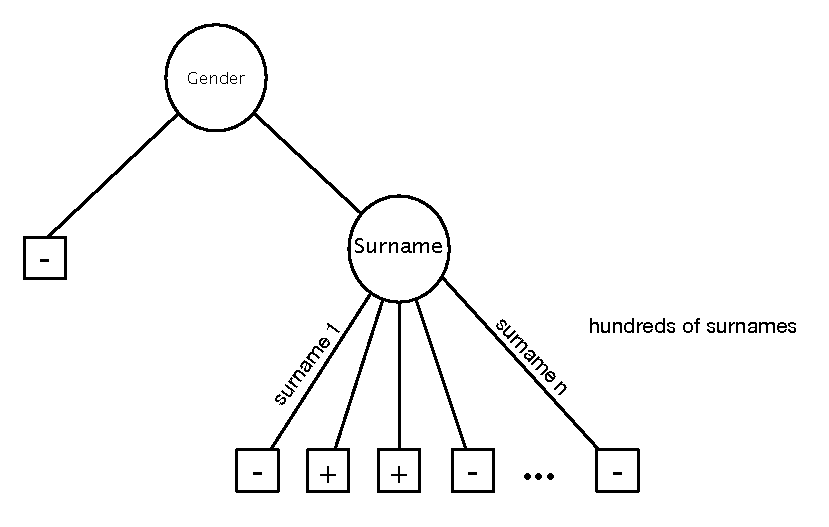
\includegraphics[width=\linewidth]{fig1.pdf}
	\caption{A decision tree for the basic features}
	\label{fig:tree_base}
\end{figure}

However, if we assume that we have access to a relational knowledge base connecting surnames to common countries of origin, we can begin to apply our feature generation technique to the problem. In the original problem, the node of female contains objects of type person. Our goal is to separate this set of people to those at high risk and those at low risk. Our recursive method defines a new learning problem with the following training set: The objects are surnames; surnames of people with the disease are labelled as positive. The features for these objects are extracted from the knowledge base.

Solving the above learning problem through an induction algorithm yields a classifier on surnames. This classifier can be used as a binary feature in the original problem. For example, it can be used as a feature in the node of female in the node of \ref{fig:tree_base}, yielding the tree seen in figure \ref{fig:lvl1_tree}. This new feature gives us a better generalization, as we now abstract the long list of surnames to a short list of countries. This also allows us to capture previously unseen surnames from those countries. However, this is not a sufficient solution, as we have no way of generalizing on previously unseen countries of origin.

\begin{figure}
	\centering
	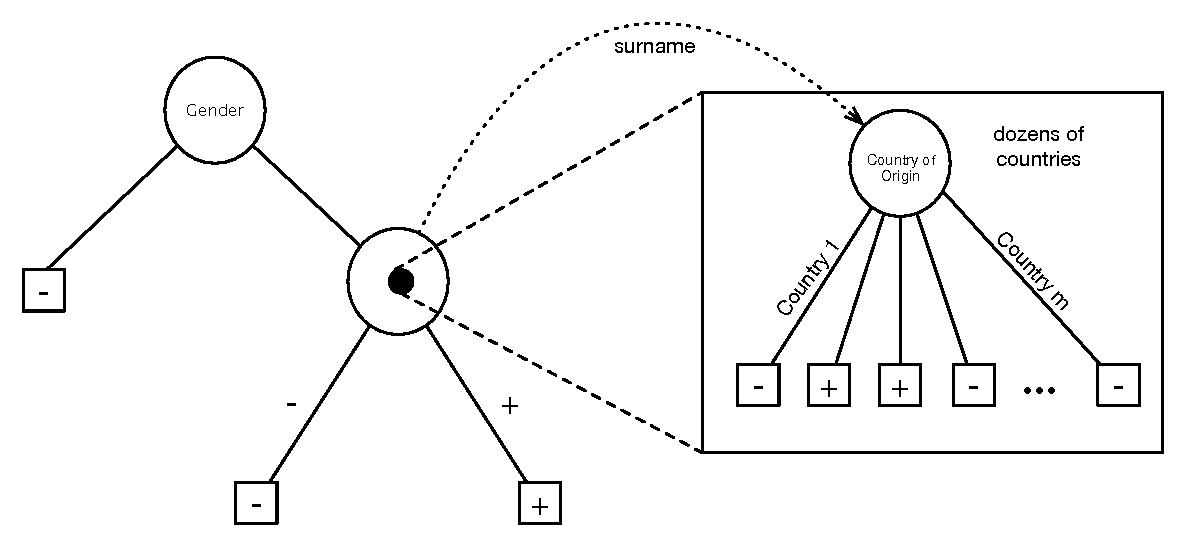
\includegraphics[width=\linewidth]{fig2.pdf}
	\caption{A constructed feature used within a decision tree}
	\label{fig:lvl1_tree}
\end{figure}

Suppose then, that we also have access to a knowledge base of facts about countries, such as average temperature, precipitation, and more (one such knowledge base is DBpedia). Using such a knowledge base, we can recursively apply our method while trying to learn the new problem. We create a new training set, the objects of which are countries of origin, and countries of surnames of people with the disease are labelled as positive. Note that this is a second level of recursion. This training set is given to an induction algorithm using the relational knowledge base about countries to construct features. The result is a classifier that tries to separate between countries of origin of people with the disease and those without the disease. The classifier is used as a feature by the first level recursive algorithm. The whole process is depicted in figure \ref{fig:moving_to_lvl2}. The resulting two-level recursive classifier is depicted in figure \ref{fig:lvl2_tree}. This constructed feature allows us to concisely and accurately capture the target concept.

\begin{figure*}[t]
	\centering
	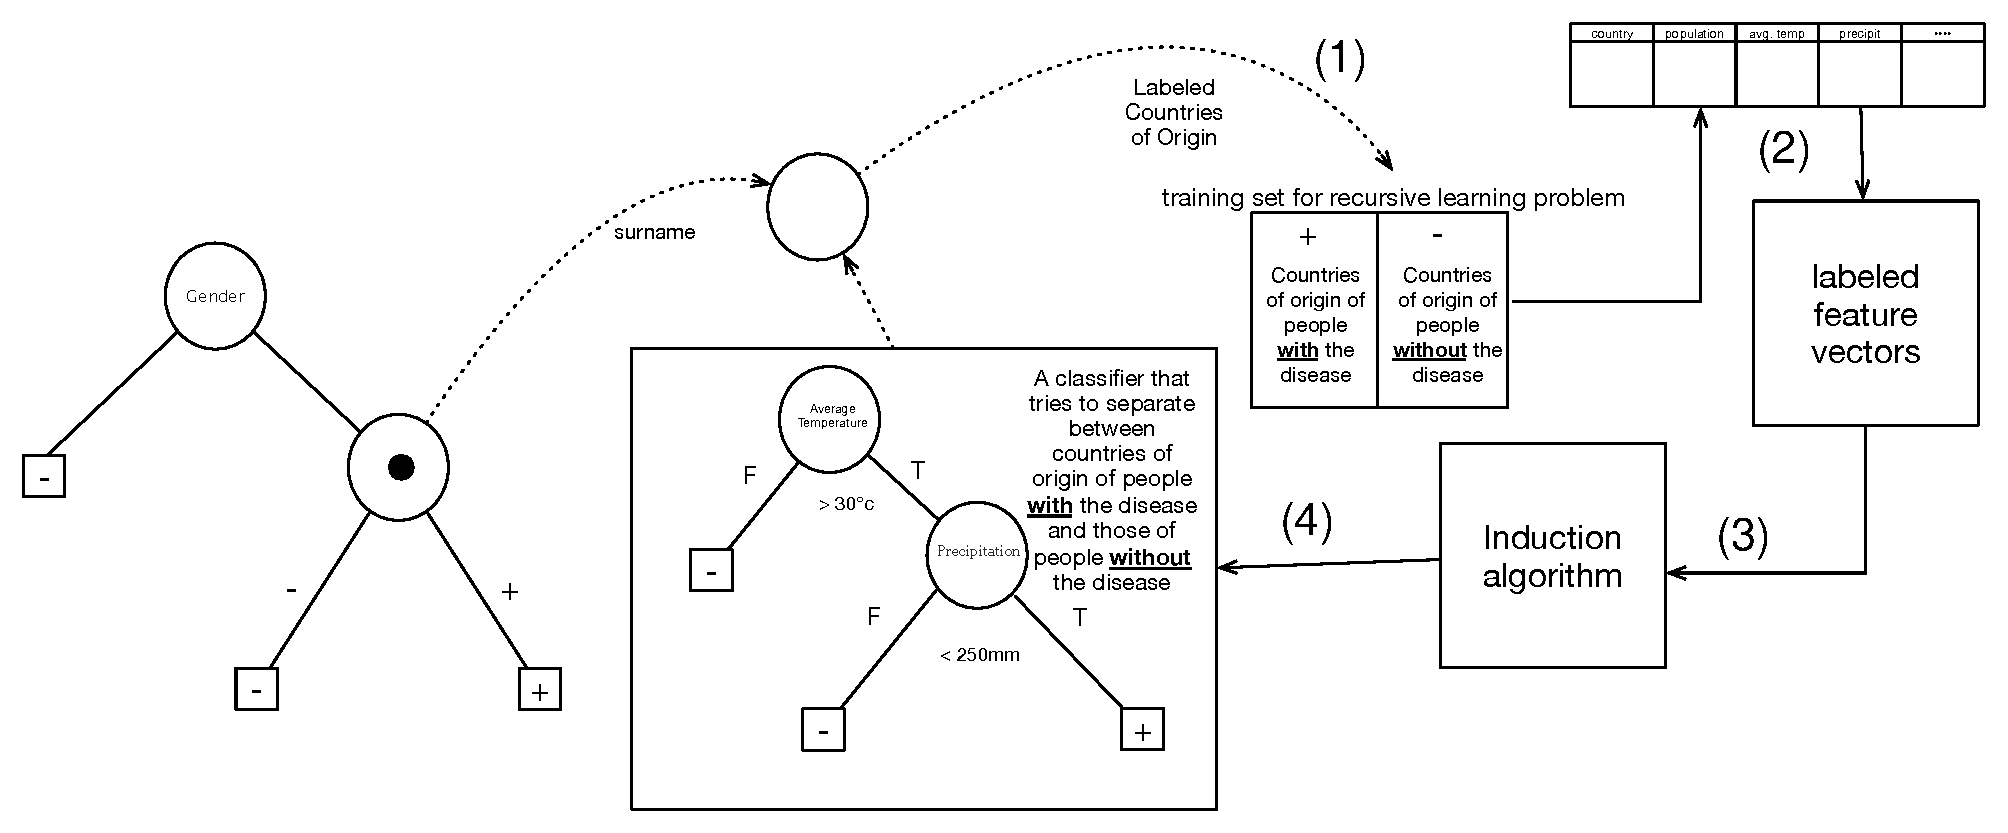
\includegraphics[width=\linewidth]{fig4_annotated.pdf}
	\caption{Recursive construction of a learning problem on countries of origin. $(1)$-Creating the objects for the new problem. $(2)$-Creating features using the knowledge base. $(3)$-Applying an induction algorithm. $(4)$-The resulting feature.}
	\label{fig:moving_to_lvl2}
\end{figure*}

\begin{figure*}[t]
	\centering
	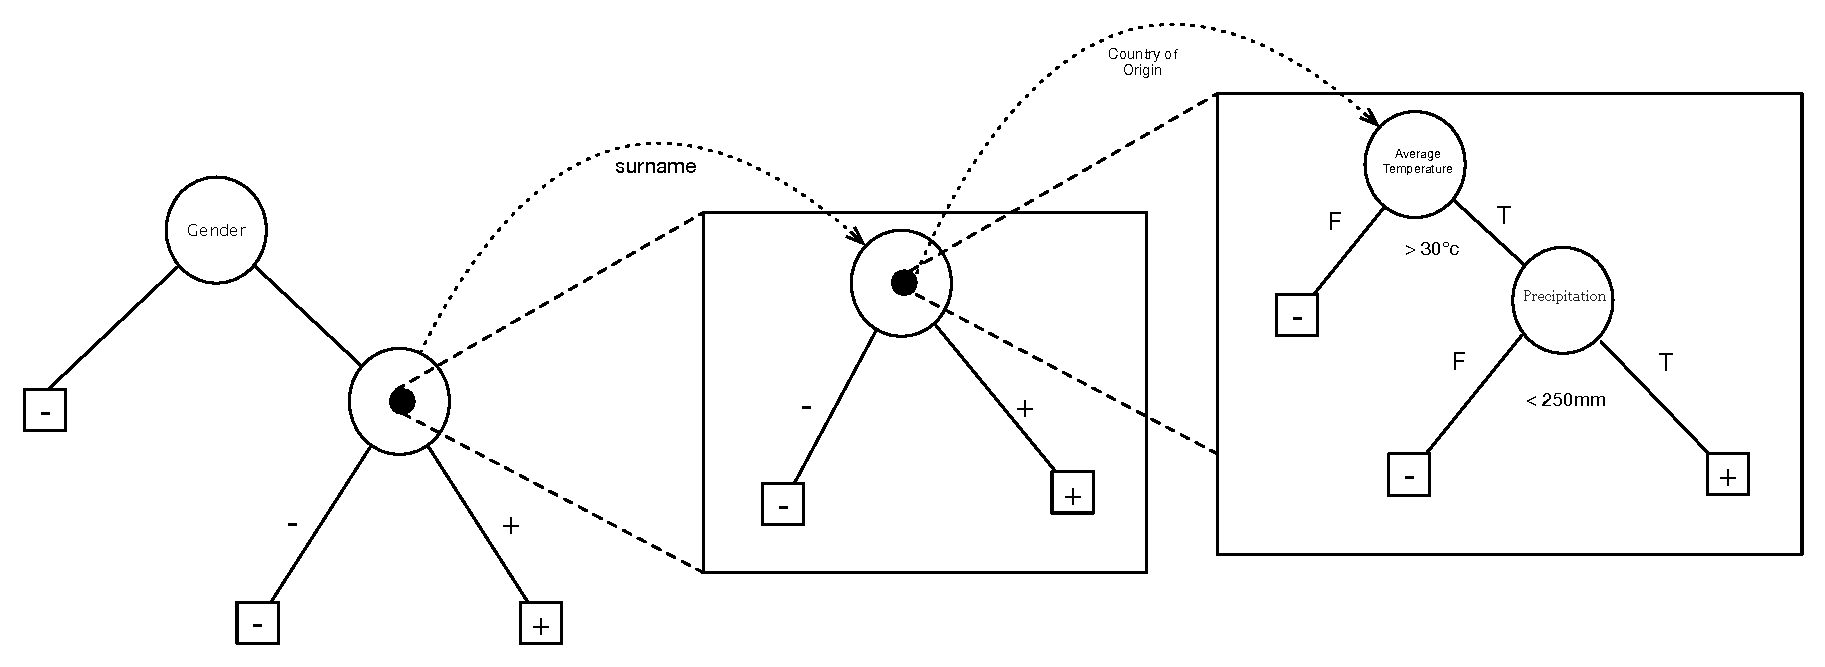
\includegraphics[width=\linewidth]{fig3.pdf}
	\caption{A two-level constructed feature used within a decision tree}
	\label{fig:lvl2_tree}
\end{figure*}


%%%%%%%%%%%%%%%%%%%%%%%%%%%%%%%%%%%%%%%%%%%%%%%%%%%%%%%%%%
%\section{Background} \label{background}
%%%%%%%%%%%%%%%%%%%%%%%%%%%%%%%%%%%%%%%%%%%%%%%%%%%%%%%%%%

%One of the earliest methods of utilizing relational information is \emph{Inductive Logic Programming(ILP)} \citep{quinlan1990learning, muggleton1991inductive}. This approach induces a set of first-order formulae that define a good separation of the given training set.
%Following this work, Relational Learning - techniques designed to utilize relational databases, have become increasingly prevalent. One such technique is that of View Learning \citep{davis2005view}, which generated new tables from existing ones, effectively performing feature generation for relational methods.

%One major attempt at adding relational knowledge to traditional induction algorithms was \emph{propositionalization} \citep{kramer2000bottom}: Since we wish to allow the use of first-order predicates in propositional methods, we create possible (non recursive) first-order predicates in a process known as refinement search \citep{van1998completeness}.
%We define a graph of possible first-order formulae by selecting an initial relation and allowing one of two possible refinement operators: The first operator is binding a single variable in the formula by assigning a constant value to it, and the second is binding a single variable using another relation.

%These operators define a search space. For each formula, we can ask whether a given object satisfies it, giving us a binary query for the data. We often prefer to only use formulae with one unbound variable, as it simplifies the satisfaction check.
%It is important to note that each application of refinement operators yields a formula that is subsumed by the parent, meaning that any object satisfying the child formula will also satisfy its parent.

%A major setback of this process is that it generates an impractically large number of features, most of which irrelevant.  To this end, \emph{upgrade} methods such as ICL \citep{van2001upgrade} were suggested, where instead of creating predicates a-priori, we do so during the training phase, allowing us to avoid searching non-promising refinements.

%As a continuation to this trend, \citet{popescul200716} suggest SGLR, an upgrade method which allows the generation of nominal attributes by using aggregation operators. Essentially, instead of simply checking whether a first-order predicate is satisfied, we perform aggregation over all objects which satisfy it. In addition, SGRL offers an initial insight into the issue of improving the search process by using Akaike's information criteria (AIC, see \citet{burnham2002model}) to select features based on a combination of complexity and predictive power.

%In the case where this external knowledge is organized as a set of relations between entities, several methods can be used. One such method is using \emph{Inductive Logic Programming} \citep{muggleton1991inductive} to generate features, in a process referred to as \emph{upgrading} \citep{van2001upgrade}. This is demonstrated through the ICL algorithm, which uses a refinement graph to search for logical formulae which serve as features. The SGLR algorithm \citep{popescul200716} extends this idea to numerical features, generated using aggregation-based techniques, and then utilizes regression for inference.

%%%%%%%%%%%%%%%%%%%%%%%%%%%%%%%%%%%%%%%%%%%%%%%%%%%%%%%%%%
\section{Generating Features through Recursive Induction}
%%%%%%%%%%%%%%%%%%%%%%%%%%%%%%%%%%%%%%%%%%%%%%%%%%%%%%%%%%

Let $O$ be a set of objects. Let $Y=\{0,1\}$ be a set of labels (we assume binary labels for ease of discussion). Let $S=\{(o_{1},y_{1}),\ldots,(o_{m},y_{m})\}$ be a set of labeled examples such that $o_{i}\in O, y_{i}\in Y$. Let $F=\{f_{1},\ldots,f_{n}\}$ be a \emph{feature map}, a set of \emph{feature functions} $f_{i}:O\rightarrow Dom_{i}$.  This definition implies a training set represented by feature vectors: $\{ (\langle f_1(o_i),\ldots,f_n(o_i)\rangle, y_i) | (o_i,y_i) \in S\}$.

Given a set of relations ${\cal R}=\{R_{1},\ldots,R_{t}\}$ with arity of $n_{j}$ ($j=1\ldots t$), we can assume \text{w.l.o.g} that the first argument is a key. For each relation $R_{j}$ we define $n_{j}-1$ new binary relations where each of the first elements is the key belonging to set $K_{j}$ and the second one is another column from some domain (not necessarily one represented within the existing feature functions).
Let $\bar{R}=\{R_{1},\ldots,R_{k}\}$ be such set of binary relations, where $R_{i}$ is defined over $K_{i}\times Dom_{i}$. These relations can thus be seen as functions $R_{i}: K_{i}\rightarrow Dom_{i}$.

\begin{defn}
	A \emph{supervised feature generation algorithm} $A$ using relations is an algorithm that given $\langle S,F,{\cal R} \rangle$, creates a new feature map $F_{{\cal R}}=\{f'_{1},\ldots,f'_{l}\}$.
\end{defn}

We would like the new hypothesis space, defined over $F_{{\cal R}}$, to be one that is both rich enough to provide hypotheses with a lower loss than those in the original space, as well as simple enough that the learning algorithm used will be able to find such good hypotheses given training data.
%We would also like there to be connections between $F$ and ${\cal R}$, meaning some of the feature values of features in $F$ (when applied to objects in $S$) also exist within relations in $\cal R$.

\subsection{Generating a feature} \label{algorithm_section} %add pseudo-code in chunks!!!

Given an original feature $f_{i}:O\rightarrow Dom_i$, our algorithm will formulate a new learning task trying to separate values in $Dom_i$ appearing in positive examples of the original learning task from those appearing in negative ones.  The result of the new learning task will be a classifier
$h_{i}:Dom_{i}\rightarrow \{0,1\}$ that can label feature values of $f_{i}$. We can then define a new binary feature $f'_{i}(x)=h_{i}(f_{i}(x))$.
We name this algorithm \emph{FEAGURE} (FEAture Generation Using REcursive induction). You can see the full pseudo-code in appendix \ref{app:2}.

%TODO: figure showing some feature->problem on values->feed to blackbox->get a binary feature for O using the domain
%\begin{figure}[t]
%	\centering
%	\includegraphics[width=\linewidth]{}
%	\caption{}
%	\label{}
%\end{figure}

In order to explain how we create such $h_{i}$, let us consider a single step of the feature generation algorithm.
Given a feature $f_{i}$, we define the set of all its value in the training set $S$ as $v_i(S) = \{v | (o,y) \in S, f_{i}(o)=v\}$. In the intro example, for instance, $v_i(S)$ will be the set of all last names of patients.
We now formulate a new learning problem with the new training set
$\hat{S_i} = \{ (v, label(v)) | v \in v_i(S) \}$.
The labelling function can be, for example, defined as
the majority label: $label(v)=majority(\{y_k| \left(o_k,y_k \right) \in S, f_{i}(o_k)=v\})$.

To define a feature map over the new training set $\hat{S_{i}}$, we look for all relations in $\bar{R}$ where the domain of the key argument contains $v_i$:
${\cal G}(S,\bar{R}) = \left\{ r \in \bar{R} | v_i(S) \subseteq \{x_1 | (x_1,x_2) \in r\}\right\}$. In the intro example, one such $r$ can be a relation mapping last names to countries of origin. We then use ${\cal G}$ as a feature map for $\hat{S_i}$.
Solving this new learning problem on $\hat{S_i}, {\cal G}(S,\bar{R})$ yields our classifier $h_{i}$.
Note that during the process of learning $h_{i}$, we can once again call the feature generation procedure to generate useful features for the \emph{new} task, hence the recursive aspect of the process. We can see this in the intro example, wherein we construct a second-level problem on countries of origin to correctly identify the appropriate conditions that signify high risk countries.

\begin{algorithm}[H]
	\caption{Creating a recursive problem}
	\label{code-creating-prob}
	\small
		%insert param stuff
		\begin{algorithmic}
			\Function{CreateNewProblem}{$f_{i}$, $S$, $\bar{R}$}
                \State $v_i(S) = \{v | (o,y) \in S, f_{i}(o)=v\}$
                \State $\hat{S_i} = \{ (v, label(v)) | v \in v_i(S) \}$ 
                \Comment $label(v)$ can be, for example, the majority function.
                \State $F_{new}=\{r(v)=c| c\in Range(r), r\in {\cal G}(S,\bar{R})\}$
                \State \Comment These are features from $Dom_{i}$ to $\{0,1\}$. For each relevant relation, we use every possible value.
                \Return $\hat{S_i}, F_{new}$ 
                \Comment Our new training set and features define a learning problem.
			\EndFunction
			
		\end{algorithmic}
	\end{algorithm}

We note that in order to prevent cycles which provide no new information, we do not allow the use of any relation that is the inverse of a previously used relation. This is not a major concern, as it is often the case that even relations using similar sets of keys will have often have differing targets (so even if $R_{i}:K\rightarrow Dom_{i}, R_{j}:K\rightarrow Dom_{j}$, usually $Dom_{i}$ and $Dom_{j}$ will be dissimilar).

When performing feature generation, we often wish to evaluate the predictive power of generated features. When such evaluation is done in the context of the entire dataset, it is possible to lose the unique benefit of a potentially powerful feature. To address this phenomenon, we decided to apply our recursive feature generation algorithm in a divide-and-conquer approach through the use of a decision tree. It is important to note, however, that the features generated in this process can be used for any induction algorithm, not necessarily decision tree induction algorithms.
Using decision trees has several advantages:
\begin{itemize}
	\item We gain an innate way to evaluate and filter generated features: A feature generated in a node will be added to the final result only if it is no less informative than the existing feature with the highest information-gain ratio. 
	\item Since we repeat this process within inner nodes of the tree, we allow for the discovery of locally relevant relationships which may be difficult to pick up when looking at the entirety of the data. We use pre-pruning based on minimal leaf size to avoid creating features which are poorly supported by actual training data.
	\item Since a decision tree classifier tests features one at a time, we can easily isolate the impact of a specific generated feature.
	\item Since we use generated features in the constructed tree, we can ensure that features generated afterwards within the tree will be largely orthogonal to it, thus ensuring variety in the generated features. 
	\item Decision trees are relatively interpretable, which leads to features which are easier to understand.
\end{itemize}
Naturally, we use decision trees as the classifiers for the newly constructed learning problems as well, allowing us to easily repeat the process recursively. %This also means we can construct features which mix multiple levels of abstraction by having some of the nodes within the tree be constructed features and others be regular ones. In the intro example, we could decide that if the country of origin appropriate for a person's last name is a country at risk, we must still ask whether the person's last name is their maiden name, as the constructed feature would otherwise yield a false positive.

Finally, the features generated during the decision tree training procedure are collected and returned for use as general, black-box features which can be used along with any induction algorithm. The decision tree itself is discarded.

%TODO: pseudo-code! "using a tree to generate and evaluate features"
%\begin{algorithm}[H]
%	\caption{Using a decision tree for feature generation and evaluation}
%	\label{code-tree-thing}
%	\small
		%insert param stuff
%		\begin{algorithmic}
%			\Function{}{}
%			\EndFunction
			
%		\end{algorithmic}
%	\end{algorithm}

The aforementioned feature generation approach offers some unique contributions:
\begin{itemize}
	\item By moving our domain space when constructing a new problem, we essentially look at the problem from another perspective, which allows for the discovery of complex relationships.
	\item The process of re-labeling allows noise reduction and emphasizes more general trends within the data that may be harder to otherwise notice.
	\item We can exploit the power of existing, well-developed learning algorithms when we create a classifier, and possibly use different ones as we take recursive steps.
	\item By using a decision tree, we can find locally good features, which often translate to globally good features.
\end{itemize}


\subsection{Applications for Text Categorization}
In order to apply our feature generation technique to the domain of text categorization, we make the standard assumption that our basic features are the words that appear in the texts, as in the bag-of-words \cite{Wu:1981:CST:1013228.511759,salton1983introduction} approach. We can therefore take words which also exist as entities within the relational database as feature values $v_i$ for the sake of our approach. To successfully do so, we naturally turn to \emph{Named Entity Recognition} (NER) approaches in order to better locate such entitles within the text.

The resulting features will locate sets of words which are connected in the relational domain. This allows us to better generalize compared to the standard bag-of-words method, and find potentially complex semantic relationships, especially when using Semantic Linked Data as our relational database.

An important side effect of this usage is that, since each label in the semantic data defines a relation and texts may contain words from different contexts, there are often multiple relations which apply and thus ${\cal G}(S,\bar{R})$ is often large. For example, a text referring to William Shakespeare's play of ``Hamlet" may connect to relations on people (for William Shakespeare himself), on theatre plays (for ``Hamlet"), and possibly locations (for the country of Denmark, where the play is set).
In order to make the process more computationally tractable, especially if it is performed recursively, we choose a sub-sample of ${\cal G}(S,\bar{R})$ for which we construct new learning problems. For the initial level of recursive activation we do so uniformly. In later levels we perform a weighted sampling on applicable relations in $\bar{R}$ based on the mean information-gain ratio of features within the current level: We take all features in current level for some relation $r\in\bar{R}$, measure the mean information-gain ratio, and use this as the weight for picking $r$ as a target for recursive activation of the FEAGURE algorithm. 

A second relevant difference to note is that generated feature may be non-applicable to a specific object, as it may be the case that none of the entities within the text come from the relation's key set \footnote{In fact, it is possible that the text contains no entities at all}. Therefore, we decided to have generated features yield a third value for cases where the generated feature does not apply.

%this entire section!
\section{Empirical Evaluation}
In this section, we discuss our experimental methodology and display our main results.
\subsection{Methodology}
%We have evaluated our method on the TechTC-100 collection \cite{gabrilovich2004text}, a collection of 100 different datasets containing binary text categorization problems of varying difficulty extracted from the Open Directory Project.

%expand?
As a knowledge base, we used YAGO2 \cite{hoffart2013yago2}, omitting any relations with literal data such as dates or geographic coordinates. This served as a ``common knowledge" database. We also made limited use of type information within the database, opting to simply use it as an additional relation.
In addition, we stripped semantic information regarding entities, such as ``TV series" or ``fictional character". For each relation within YAGO2, we created both the relation itself as well as the inverse relation, and then removed inverse relations that map very few values to very many, such as the inverse of the ``has gender" relation, which maps ``male" and ``female" to all to all existing people within the YAGO database.

We used the Stanford Named Entity Recognizer \cite{finkel2005incorporatingfull} to allow entity matching. We then performed stopword elimination using NLTK \cite{bird2009natural} , removed punctuation marks and performed stemming using the Porter Stemmer \cite{van1980new}.

We ran our feature generation algorithm for both a depth of one, creating a recursive learning problem for the original problem, and a depth of two, creating recursive learning problems for the original problem and the first order recursive problem.

%add that this is in order to convince ourselves of effectivness
We compared the new set of features (our new features combined with the original features) to the binary bag-of-words features at various feature selection levels. We used information gain ratio as the feature selection criterion.

%In order to assert that the more complex features are indeed useful, we compare to a unsupervised approach of feature generation. we used an approach similar to that of paulheim2012, blah entity recognition blah feature selection blah relational blah
%idea: what if you have basic features+this thing+our features? is it better than simply basic+this thing

\subsection{Results}
Figure \ref{fig:svm_regular} shows the accuracies achieved on all 100 datasets, using a SVM \cite{cortes1995support} classifier (Linear kernel, $C=100$), comparing the accuracy of the baseline using only the original features to a combined pool of original and generated features (with a depth limit of two). In both cases, feature selection was performed, leaving only $20\%$ of the features. The $y=x$ line represents a case where there was no change in performance, and any point above that line represents a dataset upon which we have attained an improvement. In addition, we show lines representing a $5\%$ and $10\%$ difference in accuracy. Results for a feature selection level of $10\%$ are similar, and are also statistically significant $(p<0.05)$. Results for comparing depth one and the baseline approach show similar results and were thus omitted for the sake of brevity.

\begin{figure}[]
	\centering
	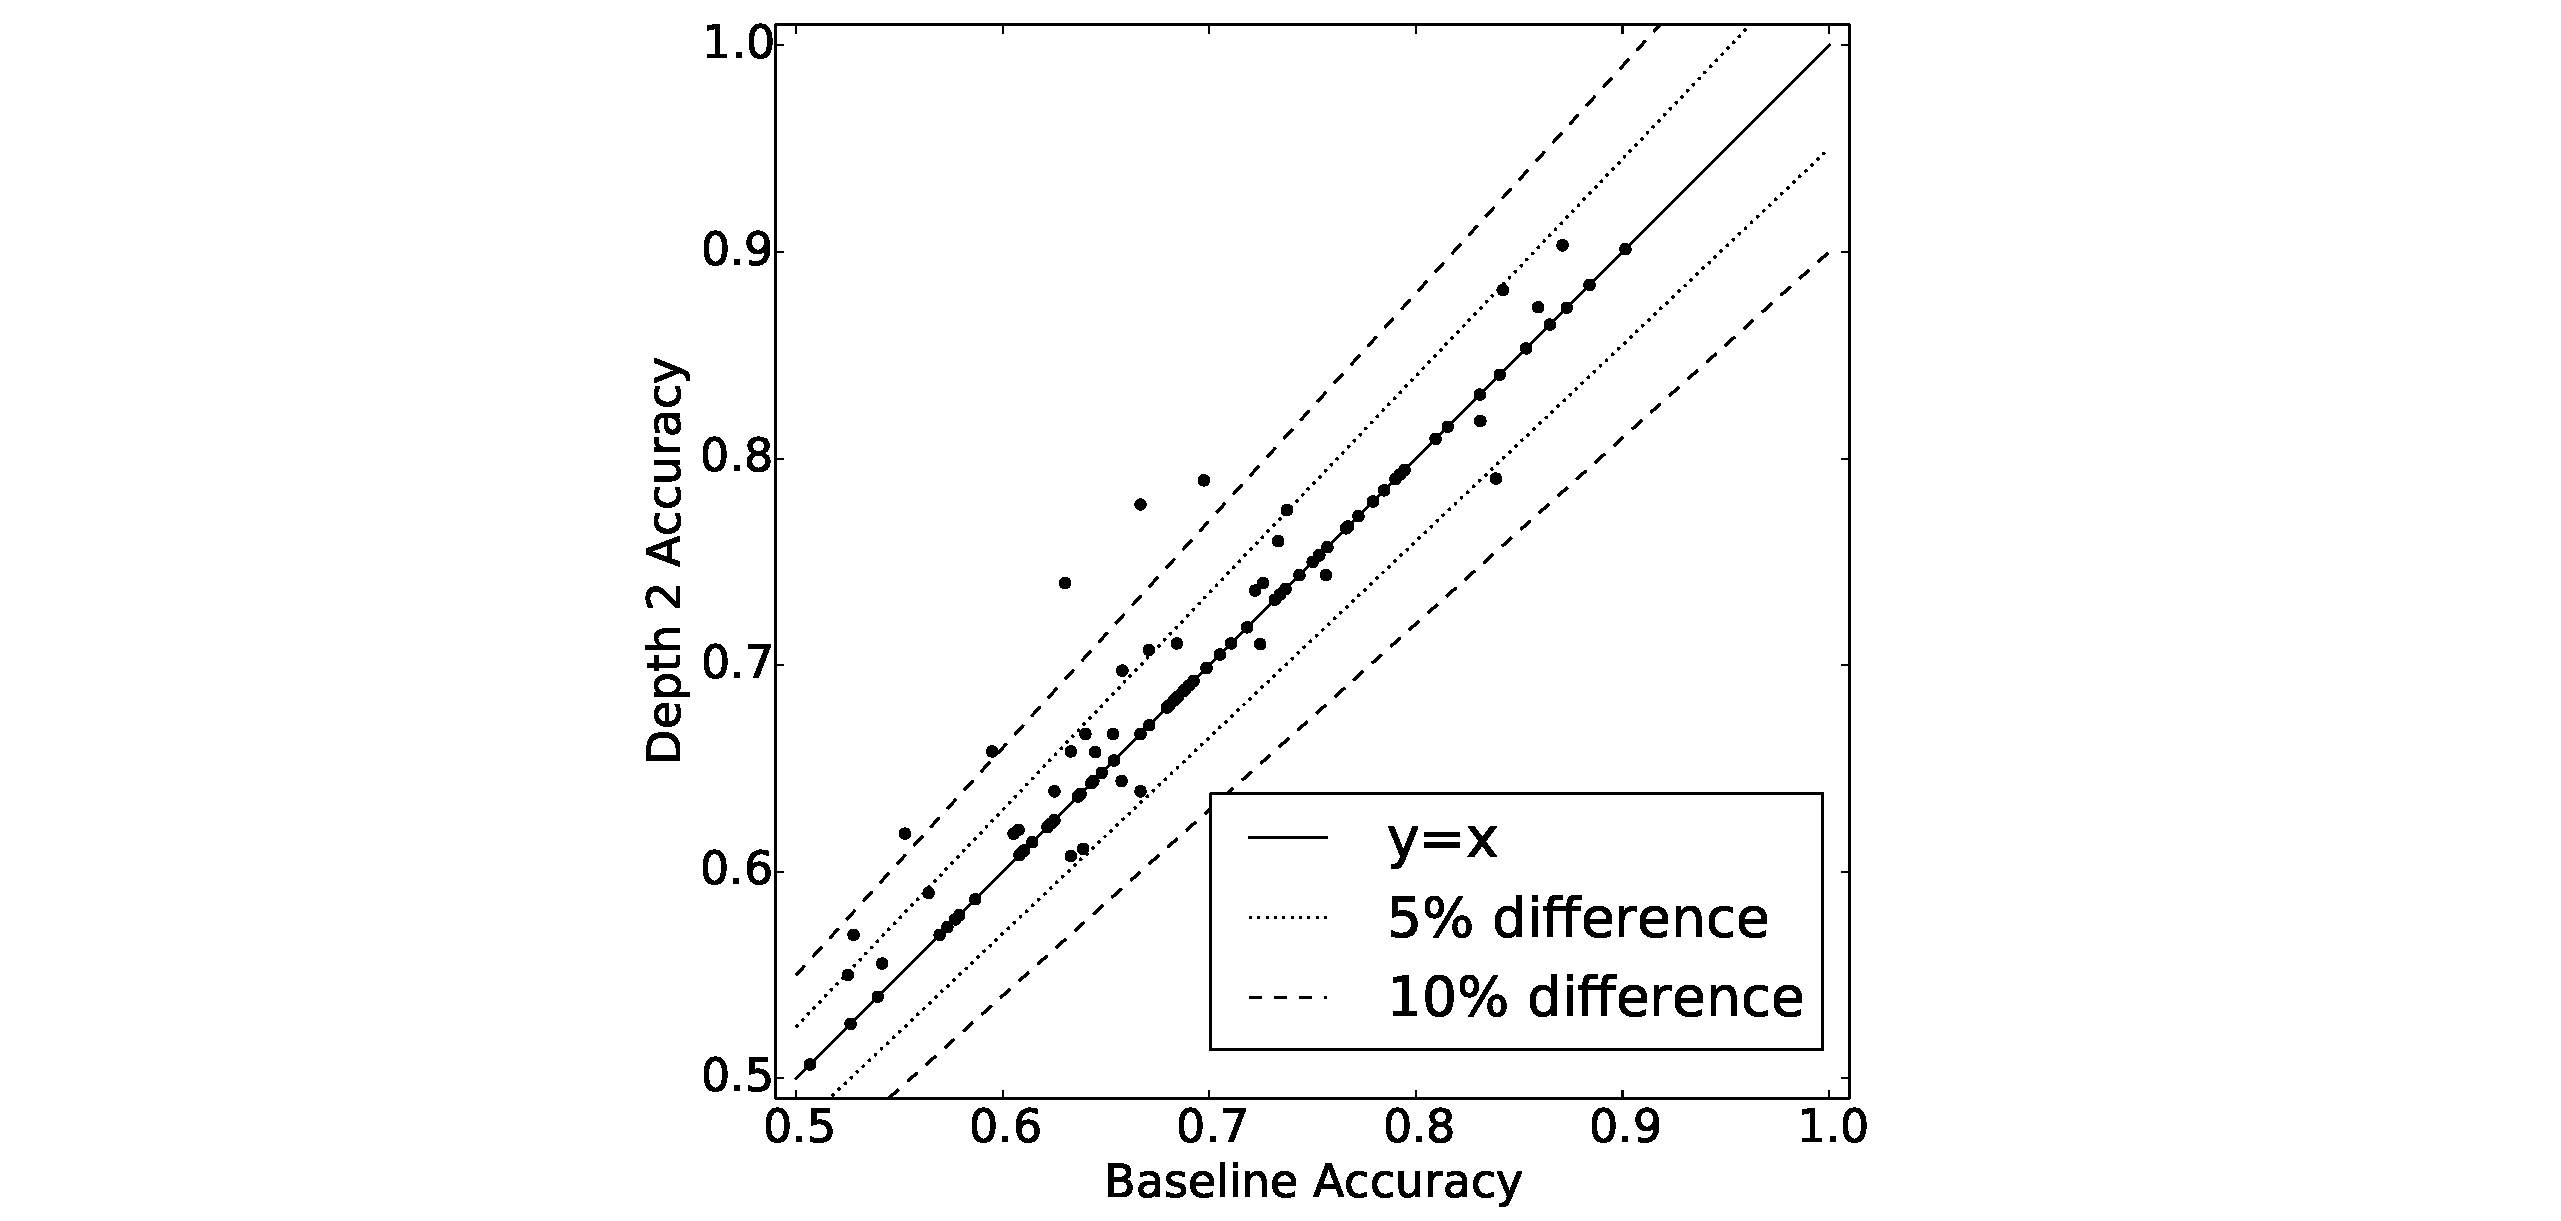
\includegraphics[width=\linewidth]{svm_full.pdf}
	\caption{Accuracy (using SVM) of baseline approach compared to the depth two feature generation approach. Each point represents a dataset. The dotted lines represent a 5 and 10 percent difference in accuracy}
	\label{fig:svm_regular}
\end{figure}

We see that the results are quite positive, with many more datasets showing an advantage to the algorithm using generated features. this advantage is also statistically significant improvement $(p<0.005)$ using a two-tailed paired t-test.

One can not ignore there are many datasets where there was no change in performance. A closer look at these datasets reveals that the cause for this is that  no features were generated. Further analysis reveals that this occurs due to a large number of highly sparse recursive learning problems. Since we only sample some of the possible problems to attempt feature generation, this is a factor in the amount of features generated in general, as well as part of the reason why no features are generated for some datasets. Experiments in lowering the amount of sampled relations show a decrease in both the number of generated features and the mean increase in accuracy.

In order to test the versatility of our approach, we also tried to look at a very different type of classifier, and therefore used a K-Nearest Neighbours \cite{fix1951discriminatory} classifier ($K=1$). As before, we performed feature selection, leaving only $20\%$ of the features. The results are shown in figure \ref{fig:knn_clean}. We see a similar trend to that of SVM, albeit at a lower base accuracy level. These results also show a statistically significant improvement $(p<0.01)$ using a two-tailed paired t-test.


%any good qualtive examples

\begin{figure}[]
	\centering
	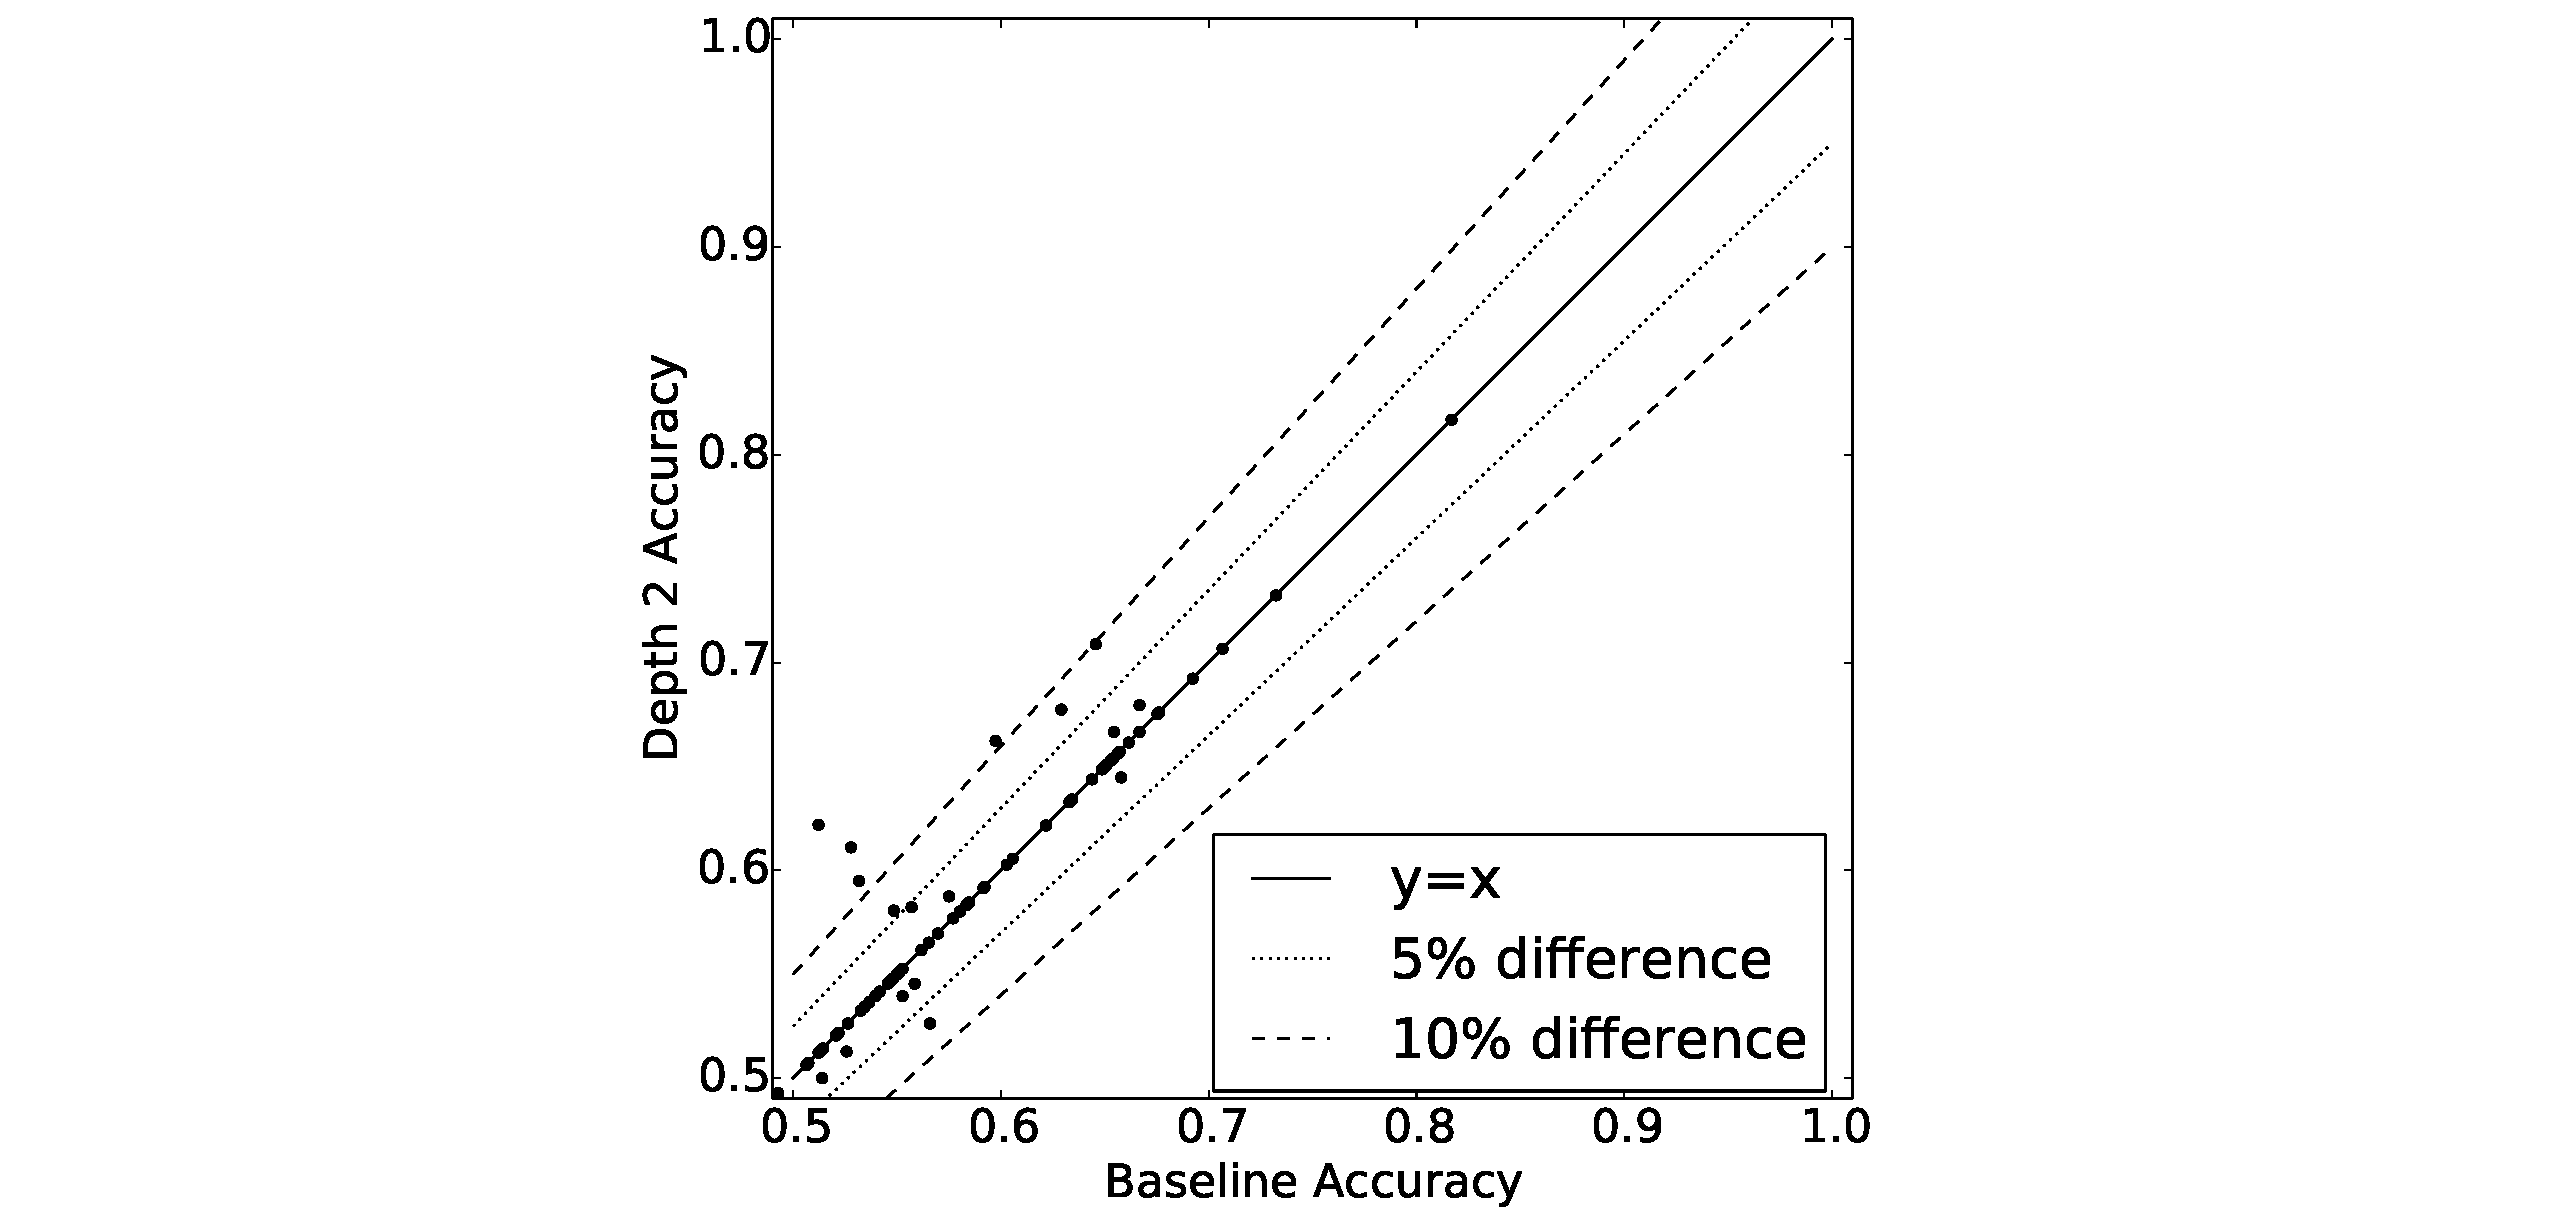
\includegraphics[width=\linewidth]{knn_clean.pdf}
	\caption{Accuracy (using KNN) of baseline approach compared to the depth two feature generation approach. Each point represents a dataset}
	\label{fig:knn_clean}
\end{figure}

%results, specific examples (qualative analysis), explaining it and so on
%Figure \ref{fig:accuracy} shows the average accuracy across all datasets within techTC-100 for various feature selection levels. We compare the baseline features to a combined pool of the original and generated features. The left graph shows the accuracy using K-Nearest Neighbours \citep{fix1951discriminatory} as our classifier ($K=1$) and the right graph shows the accuracy using SVM \citep{cortes1995support} as our classifier (Linear kernel, $C=100$). %Results ran using CART \citep{breiman1984classification} as a classifier (requiring a consistent tree) yielded no discernible pattern of improvement or decrease in performance, except in very low feature selection levels, where there is a significance decrease in accuracy $ (p<0.05) $.

%We see that the depth one application is better than the bag-of-words approach, and the depth two application yields a further improvement. We witness this for both algorithms, especially in high (over $20\%$) feature selection levels. This is slightly more apparent for SVM-based classification. Both depths achieve a significant improvement $ (p<0.05) $ over the bag-of-words approach for multiple feature selection levels. For instance, when taking $20\% $ of the features, we see a statistically significant improvement for both KNN and SVM classification accuracies (using a paired-t-test).
%Furthermore, for SVM we see a significant improvement between the first and second depths at a $0.75\%$ feature selection level. For KNN, there is a statistically improvement between the depths for feature selection levels in the range $60\%-80\%$, though the depth two application is only significantly better than the baseline approach for a feature selection level of $70\%$

%Figure \ref{fig:accuracy_low} shows the average accuracy across all datasets within techTC-100 for very low feature selection levels.
%We see that in lower feature selection levels the effect generally diminishes for both classifier types, as some of the generated features are filtered out by the feature selection process. The lowest feature selection levels at which we found a significant improvement are $0.75\%$ for SVM and $15\%$ for KNN.

%\begin{figure}[]
%	\centering
%	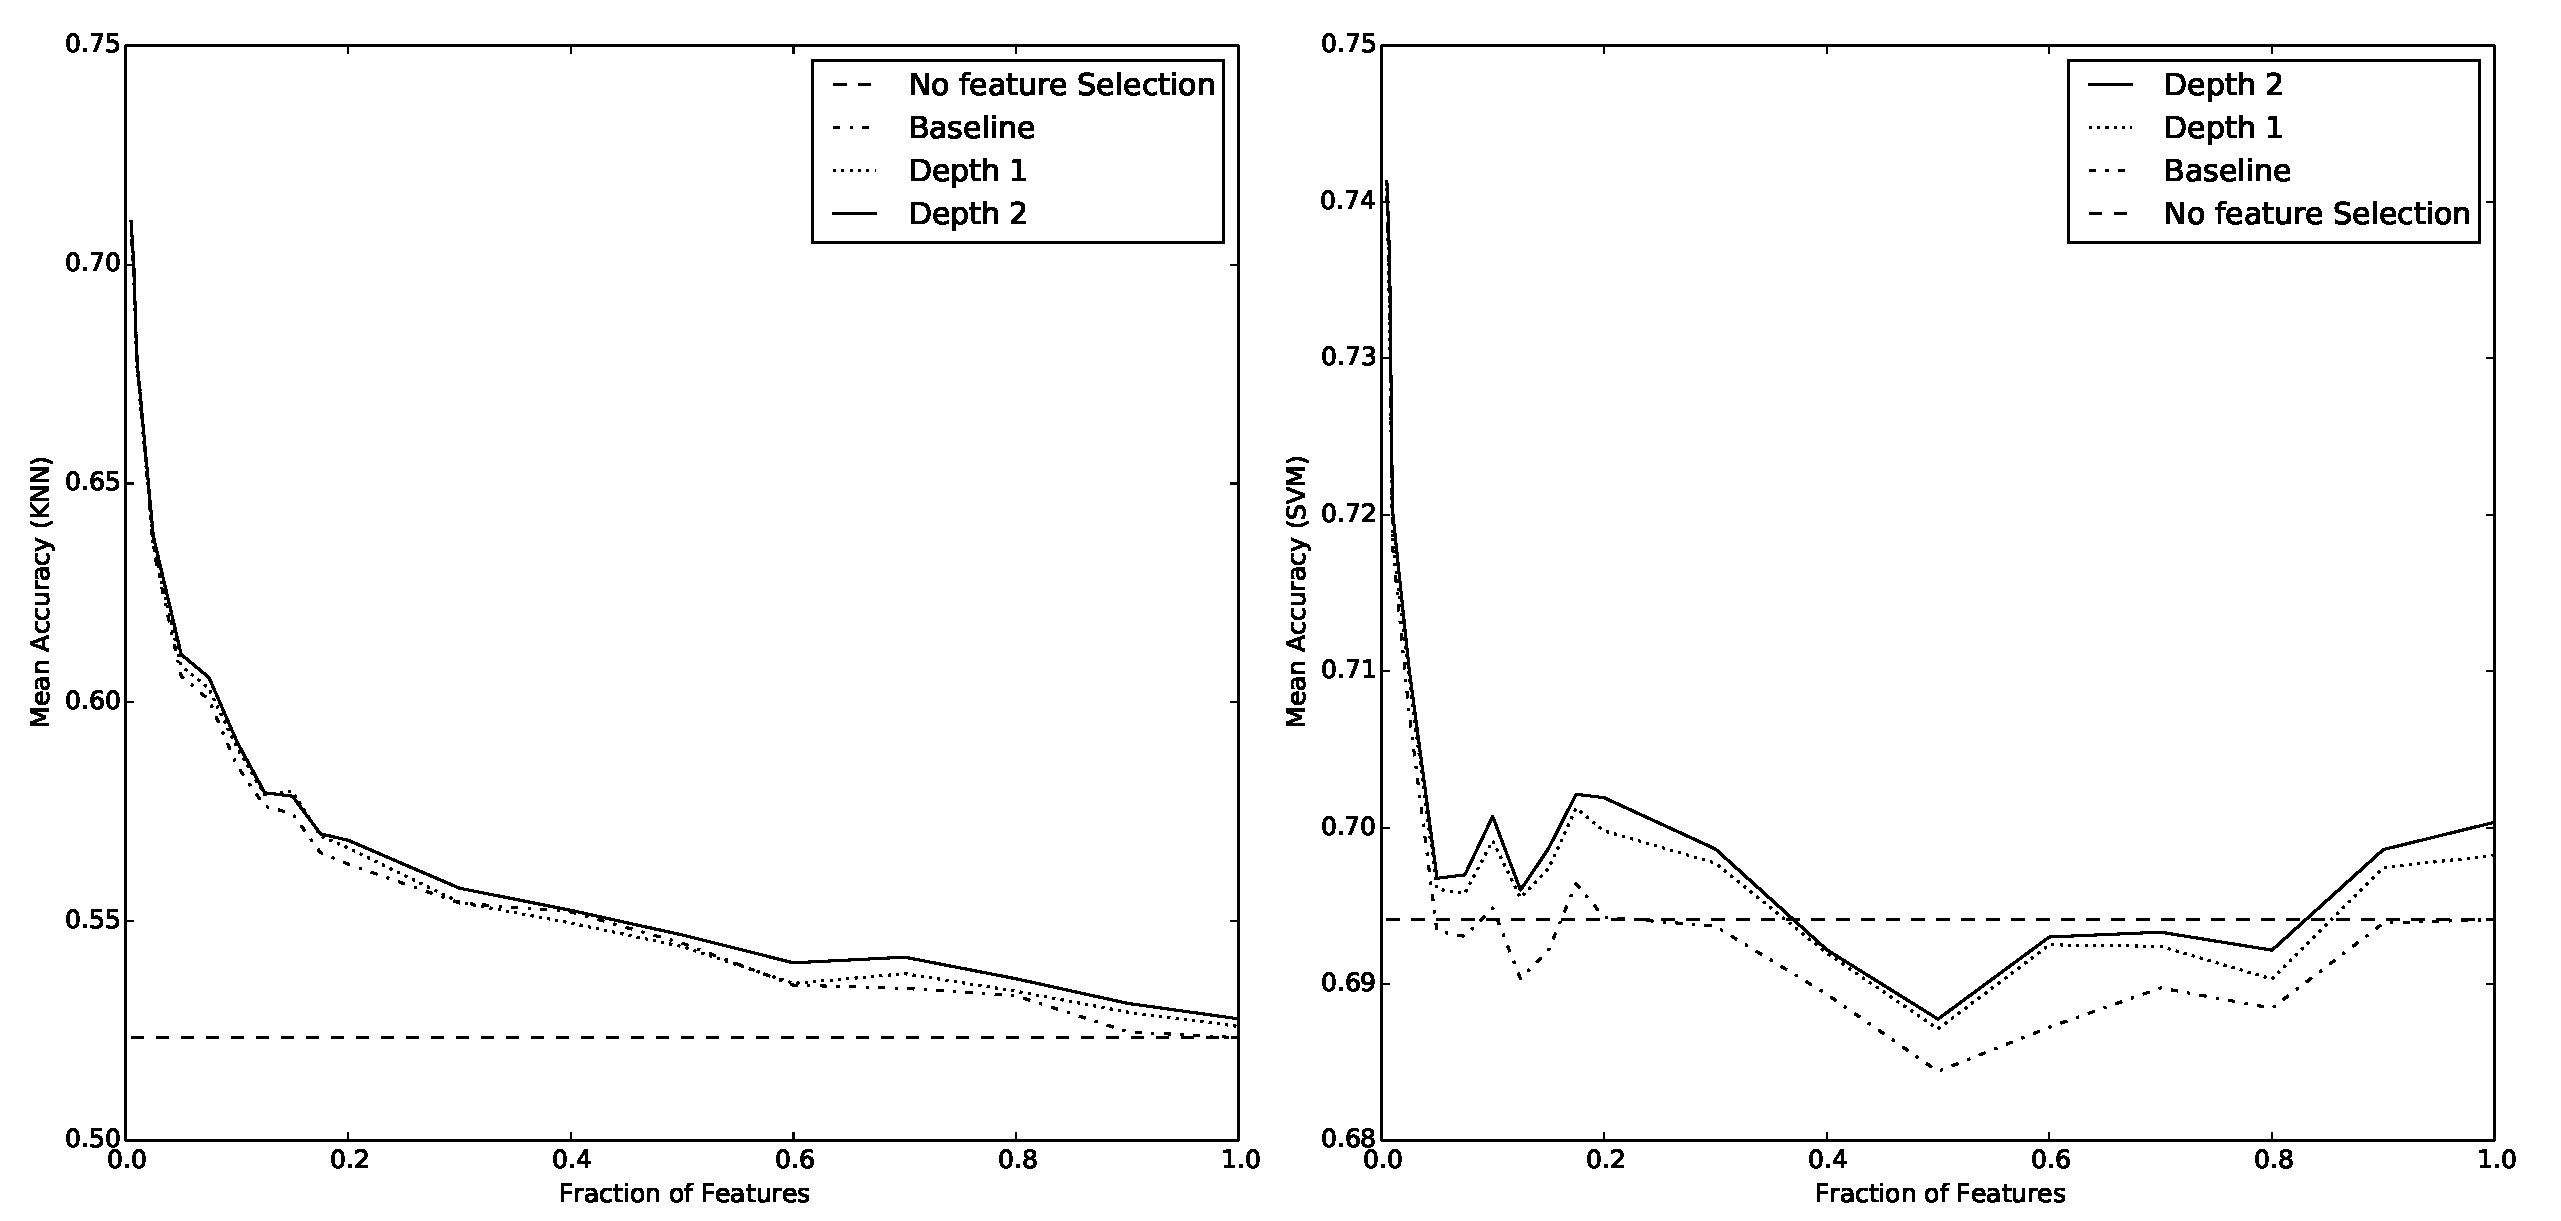
\includegraphics[width=\linewidth]{acc2.pdf}
%	\caption{Average accuracy across all 100 datasets for various feature selection levels. Left side: KNN, Right side: SVM}
%	\label{fig:accuracy}
%\end{figure}

%\begin{figure}[]
%	\centering
%	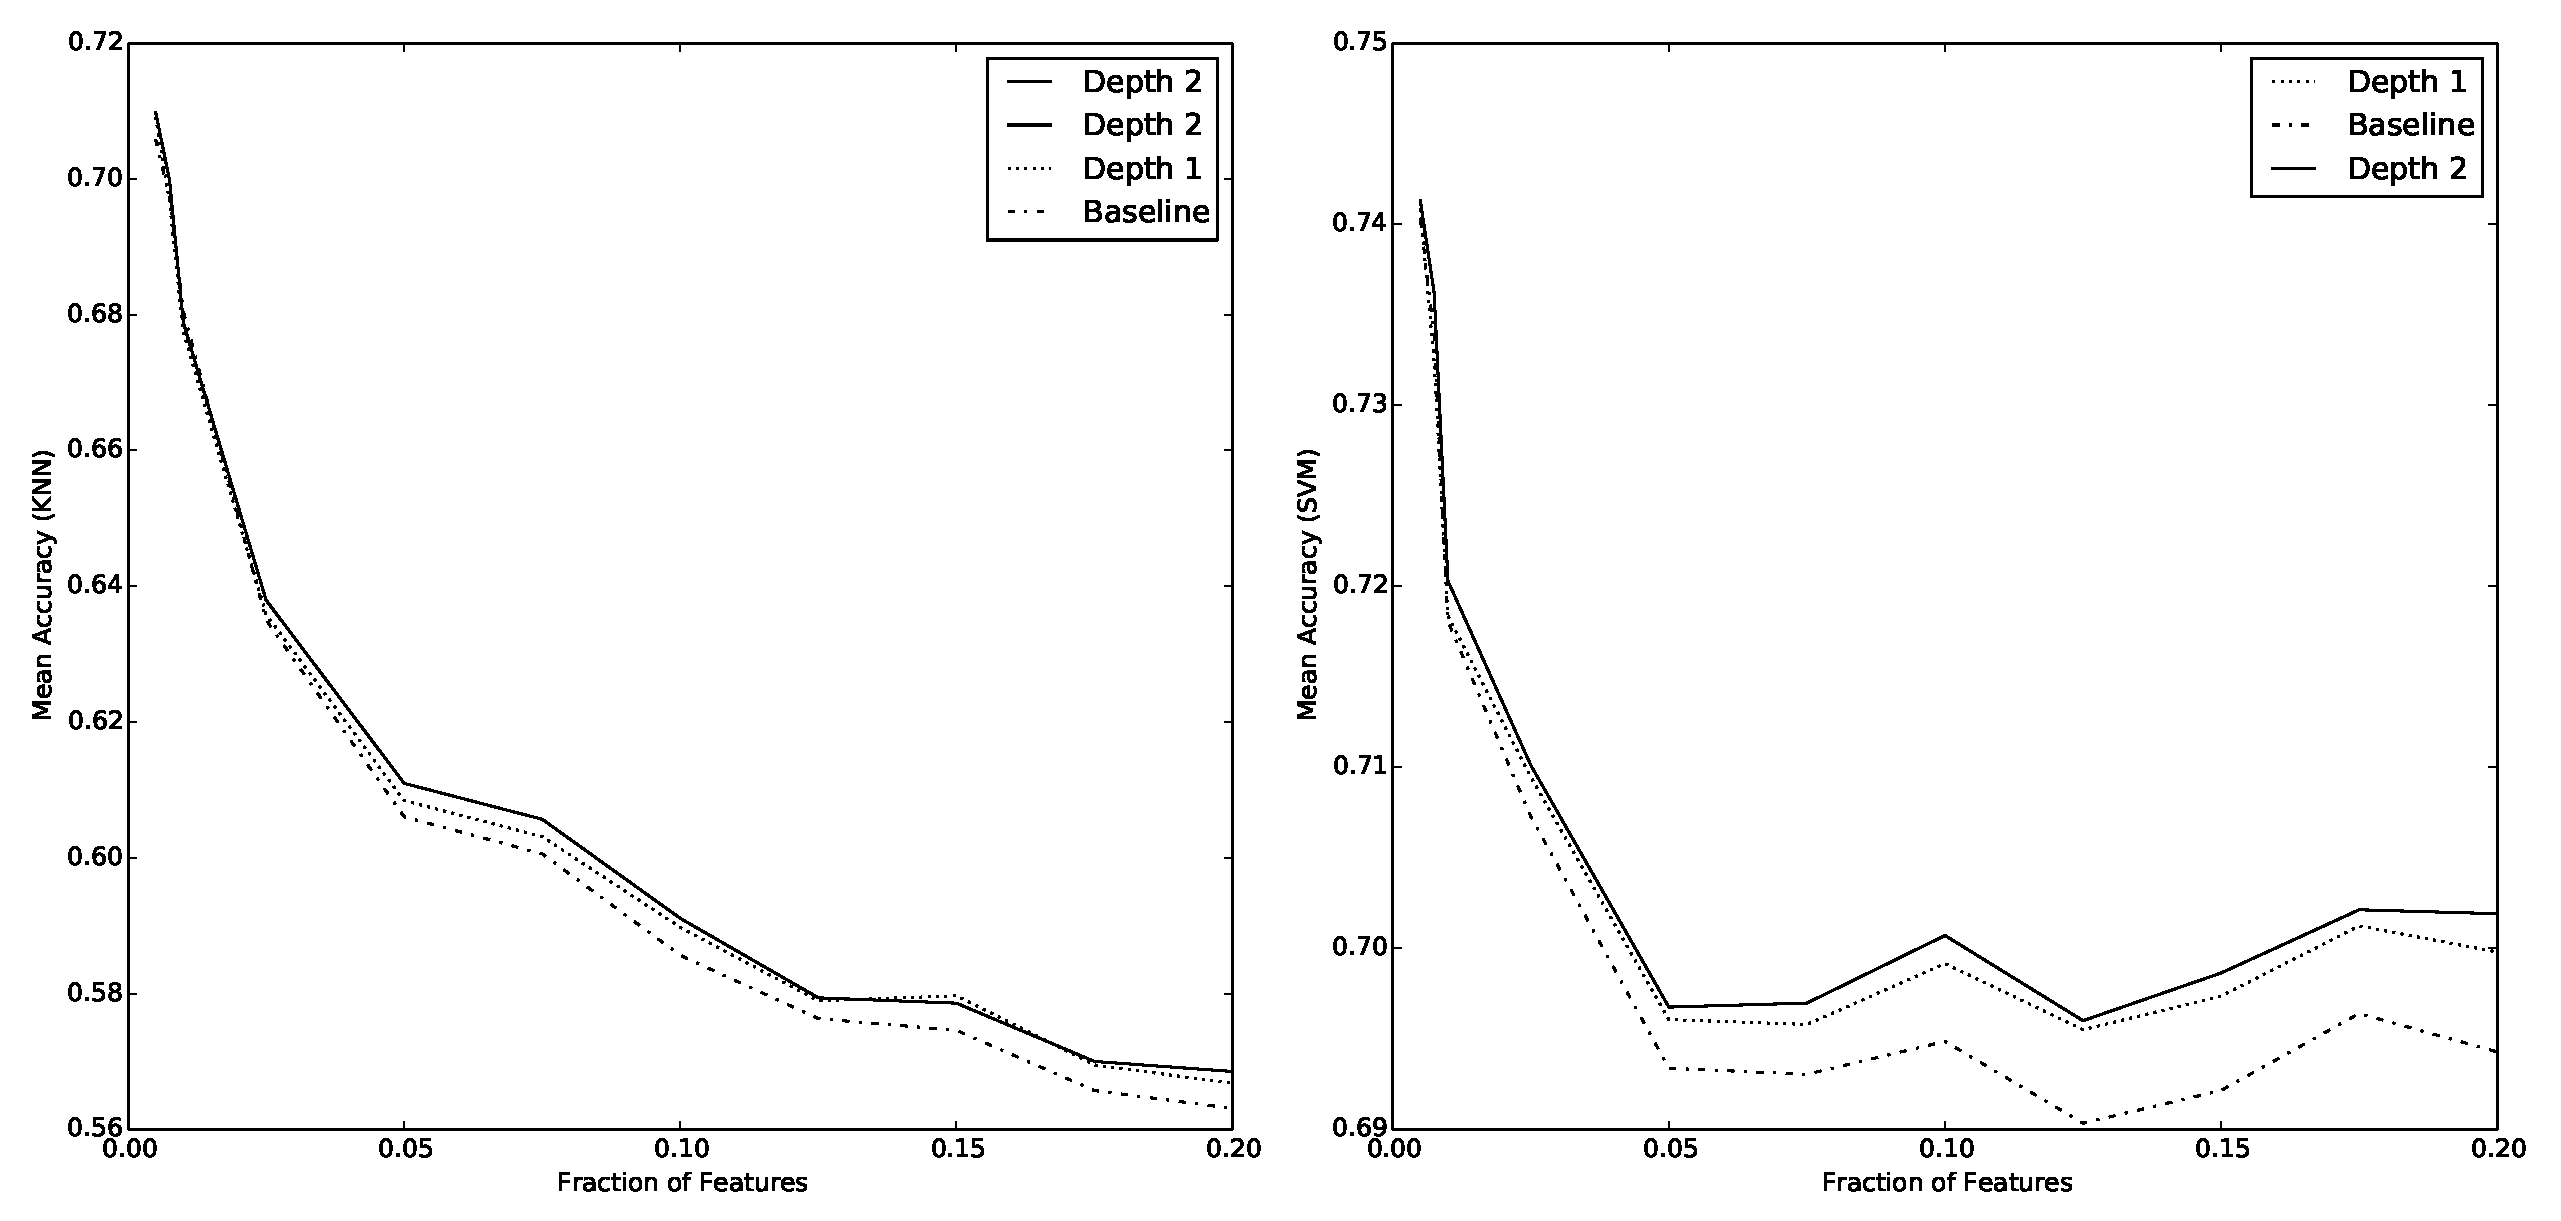
\includegraphics[width=\linewidth]{acc_low2.pdf}
%	\caption{Average accuracy across all 100 datasets for very low feature selection levels. Left side: KNN, Right side: SVM}
%	\label{fig:accuracy_low}
%\end{figure}

%We note that due to the conservative feature generation process, very few features are generated: in nearly half of the datasets within techTC-100, no features are generated at all, and in no single dataset is the number of features greater than six. We also note that most generated features arise from local contexts, i.e, when looking at the entire dataset we would have difficulty identifying these features as especially useful.

%A more careful look at datasets where no features are generated reveals that they tend to result in a larger number of highly sparse recursive learning problems. Since we only sample some of the possible problems to attempt feature generation, this is a major factor in the amount of features generated in general, as well as part of the reason why no features are generated for some datasets. Experiments in lowering the amount of sampled relations show a noticeable decrease in both the number of generated features and the mean increase in accuracy compared to results discussed above.

%Figure \ref{fig:ratios} shows the mean ratio between the accuracy of the base approach and our recursive approach across all 100 datasets, and figures \ref{fig:ratios_max} and \ref{fig:ratios_min} show the minimal and maximal ratios accordingly. We note that while the average improvement in accuracy is not large (due to many datasets where no features are generated), we can often achieve a $20\%-25\%$ increase, and potentially reach as much as a $40\%$ increase in accuracy for some datasets within TechTC-100. We also note that it is possible to have a decrease in accuracy, but that for most cases, especially when using SVM as the classification method, we can limit it to no more than a $10\%$ decrease.

%We also note that the depth one application tends to be more conservative than a depth two approach, yielding a lesser improvement on average and in the best case, but also a offers a more measured decrease in the worst cases.
%Results for CART reaffirm this notion. However, there is no clear trend regarding the mean ratios, and there is a much higher variance in terms of minimal and maximal ratios, offering as much as a $30\%$ difference in either direction.

%\begin{figure}[]
%	\centering
%	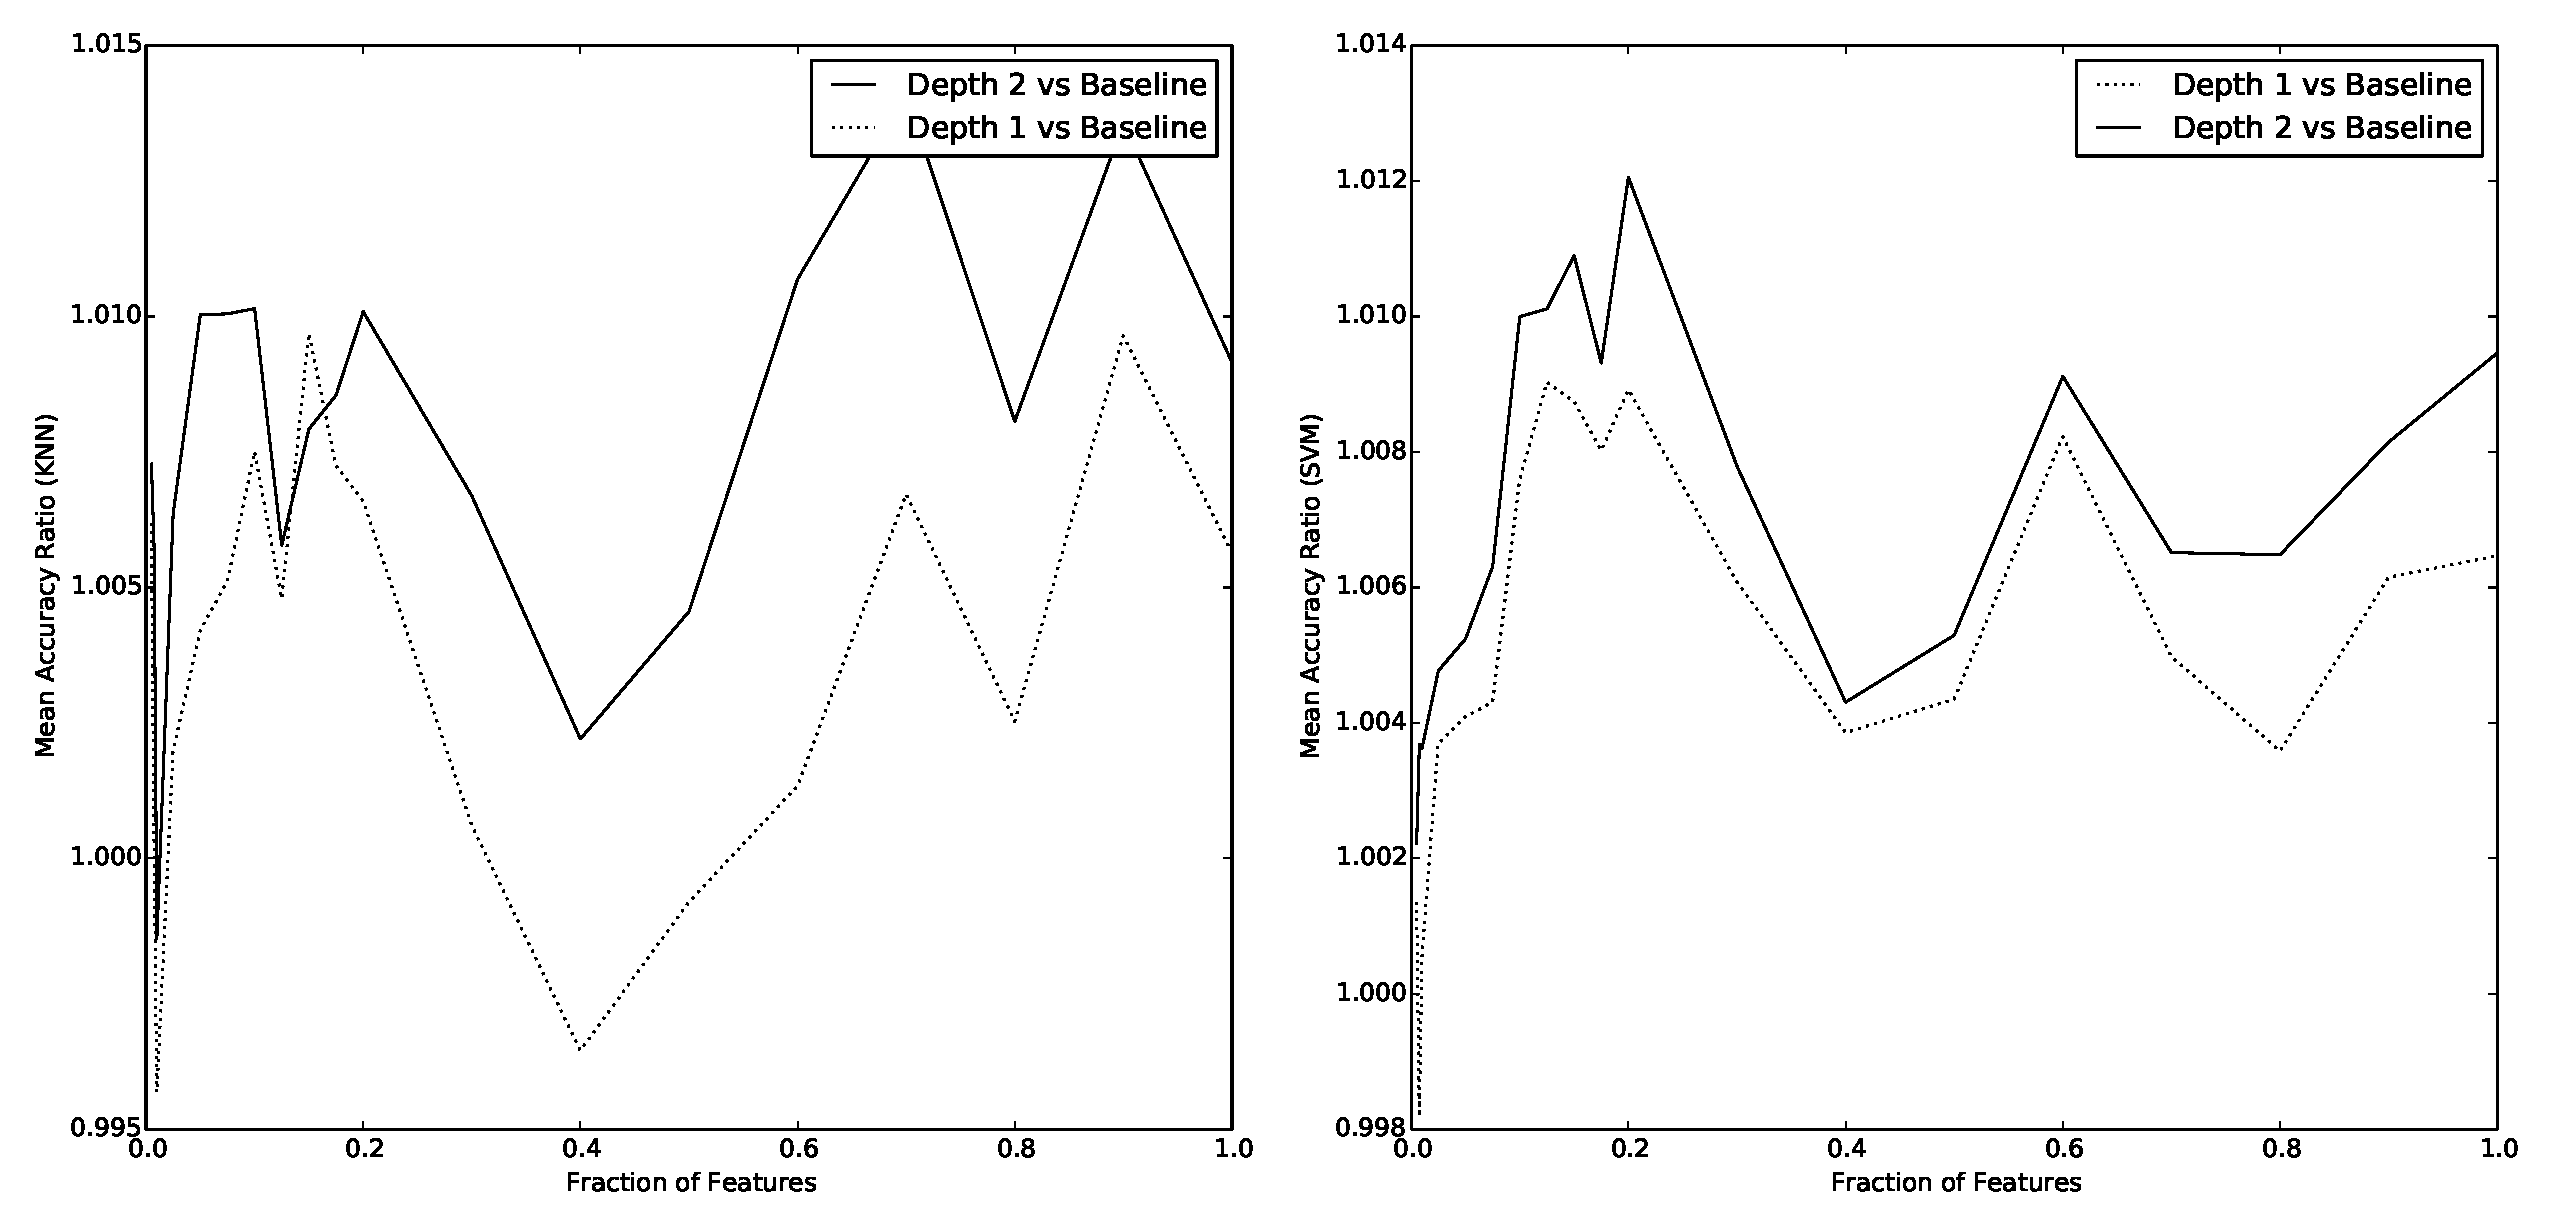
\includegraphics[width=\linewidth]{ratios2.pdf}
%	\caption{Average accuracy ratio across all 100 datasets for various feature selection levels. Left side: KNN, Right side: SVM}
%	\label{fig:ratios}
%\end{figure}

%\begin{figure}[]
%	\centering
%%	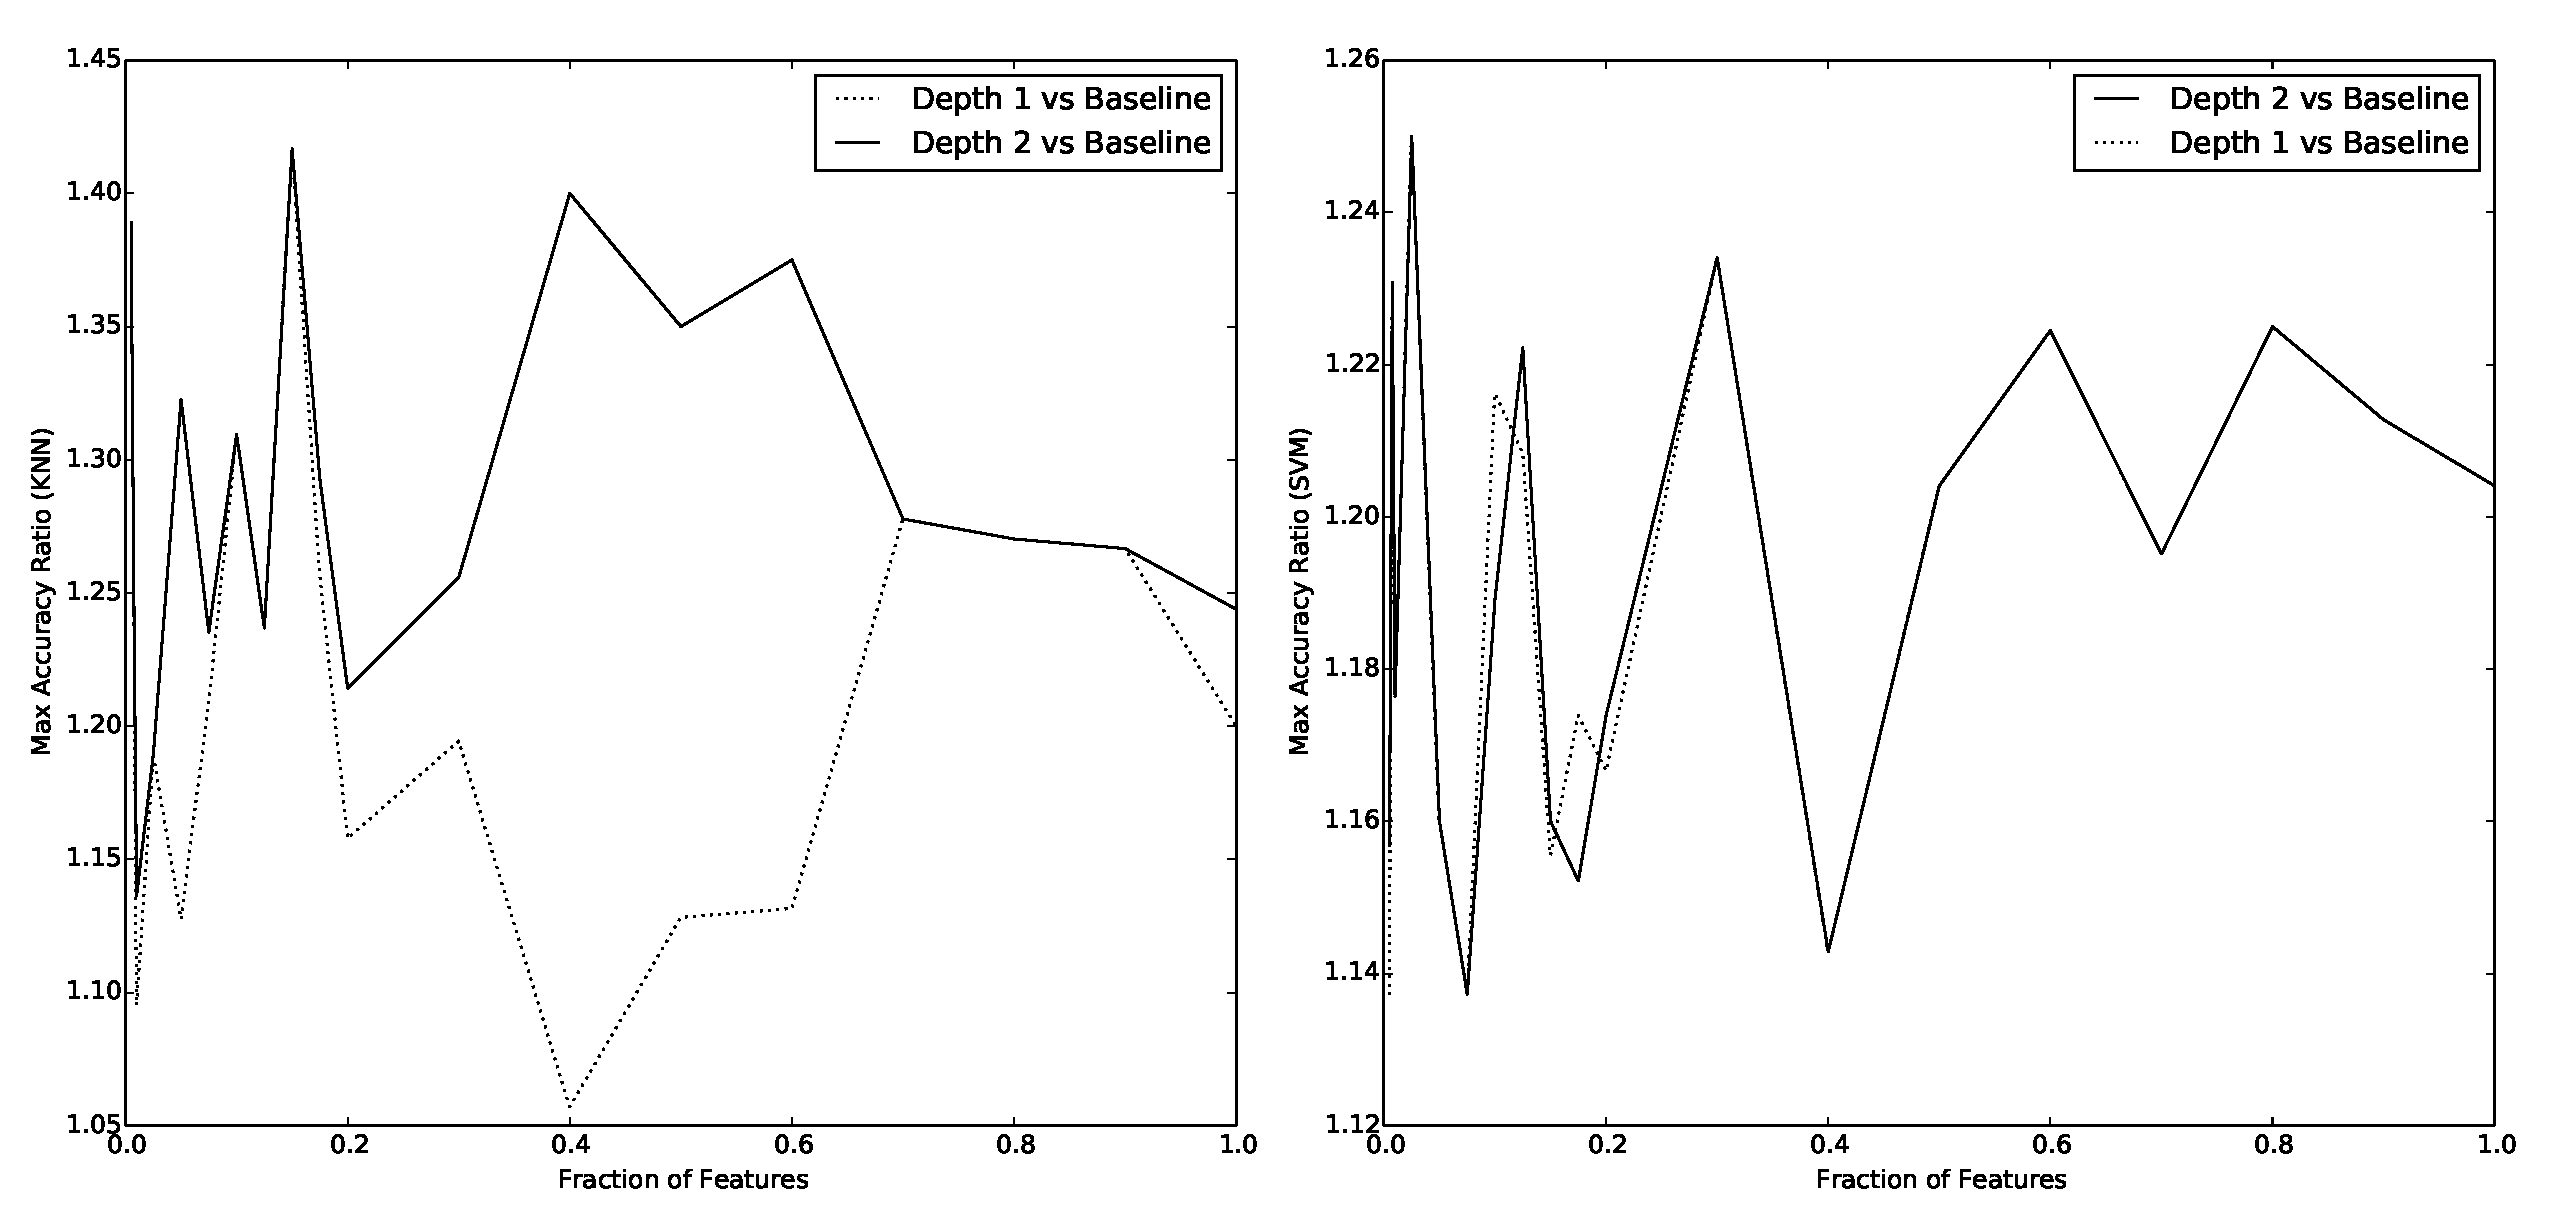
\includegraphics[width=\linewidth]{ratios_max2.pdf}
%	\caption{Maximum accuracy ratio across all 100 datasets for various feature selection levels. Left side: KNN, Right side: SVM}
%	\label{fig:ratios_max}
%\end{figure}

%\begin{figure}[]
%	\centering
%	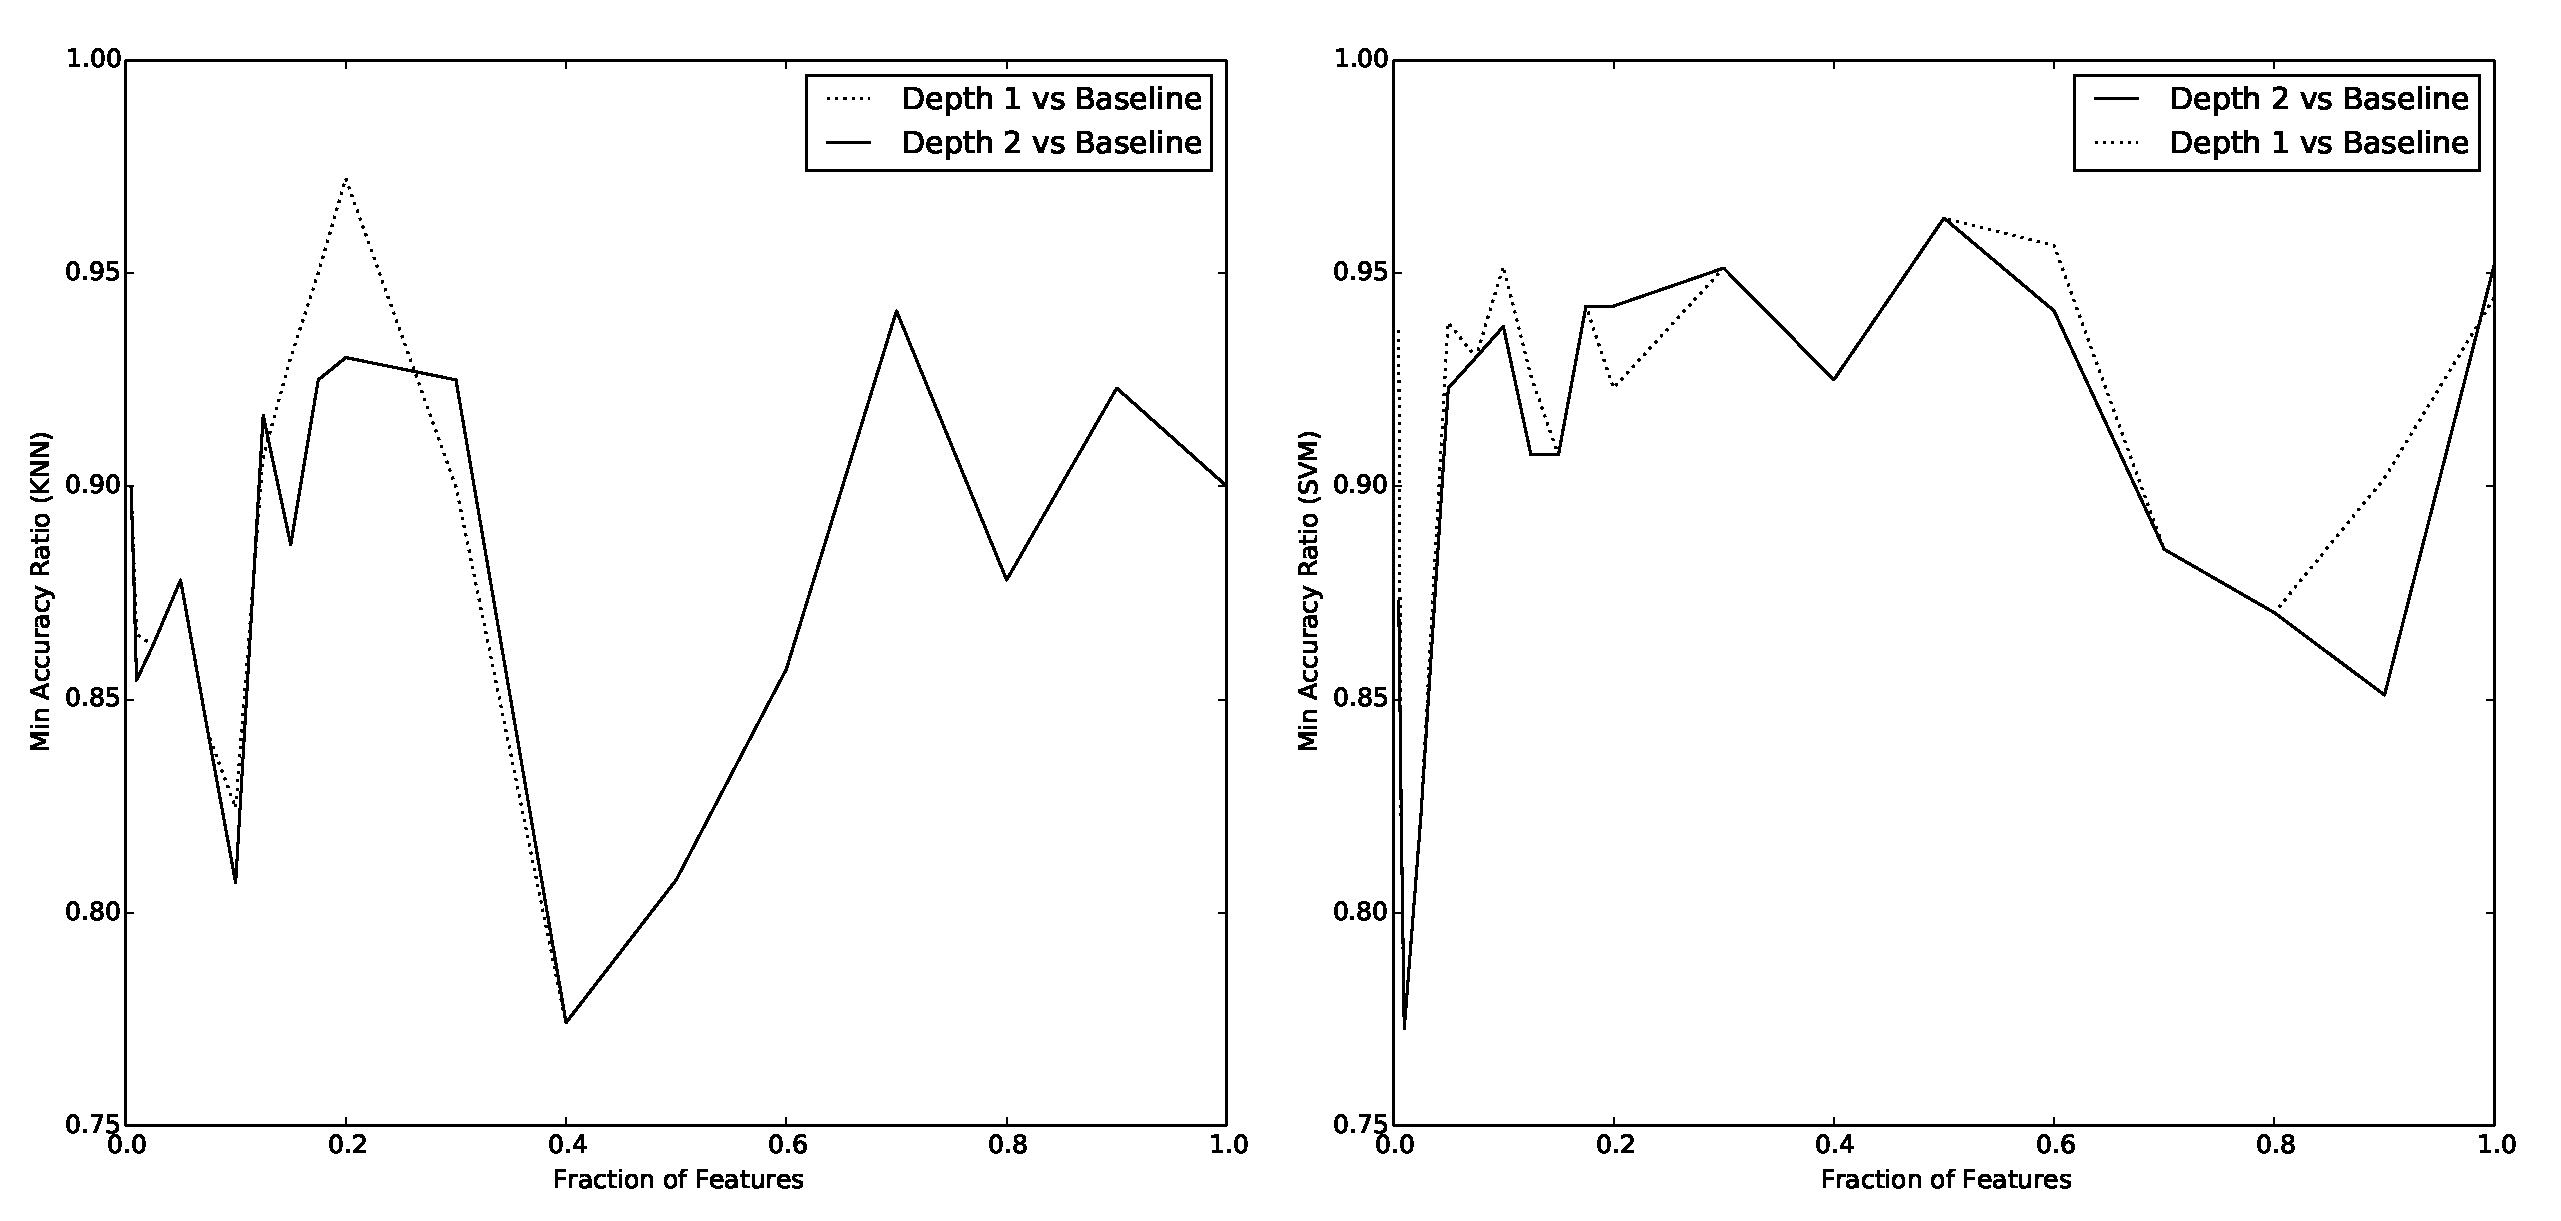
\includegraphics[width=\linewidth]{ratios_min2.pdf}
%	\caption{Minimum accuracy ratio across all 100 datasets for various feature selection levels. Left side: KNN, Right side: SVM}
%	\label{fig:ratios_min}
%\end{figure}


%\subsection{Qualitative Analysis}
%In order to better understand the contribution of these features, let us look at several of them to try and better understand them. Figure \ref{fig:level1_good} shows one of the features generated for single level feature generation. We can see that the feature attempts to separate based on geographical location. Figure \ref{fig:level1_simple} shows a simple feature regarding people, and showcases the fact that when there is no need for overly complex features, our technique will not force such features. This feature yields a $10\%-15\%$ increase in accuracy (depending on feature selection level), and is generated by both the single and two level approaches.

%Figure \ref{fig:level2_tree} showcases the additional power of the level two approach. The second level learning problem separates non-countries from countries, as well as countries which deal with non fuel manufacturing Arabic nations from those who embargo them.

%Figure \ref{fig:weird_trees} showcases some of the unique oddities of using our technique with the YAGO2 knowledge base. Since YAGO groups together all entities which have a grammatical gender (including fictional characters and non-living objects) under a single relation, the constructed feature looks at both deceased individuals and words that are the same as Australian television channels (such as Gold and Galaxy) at the same time.

%\begin{figure}[]
%	\centering
%	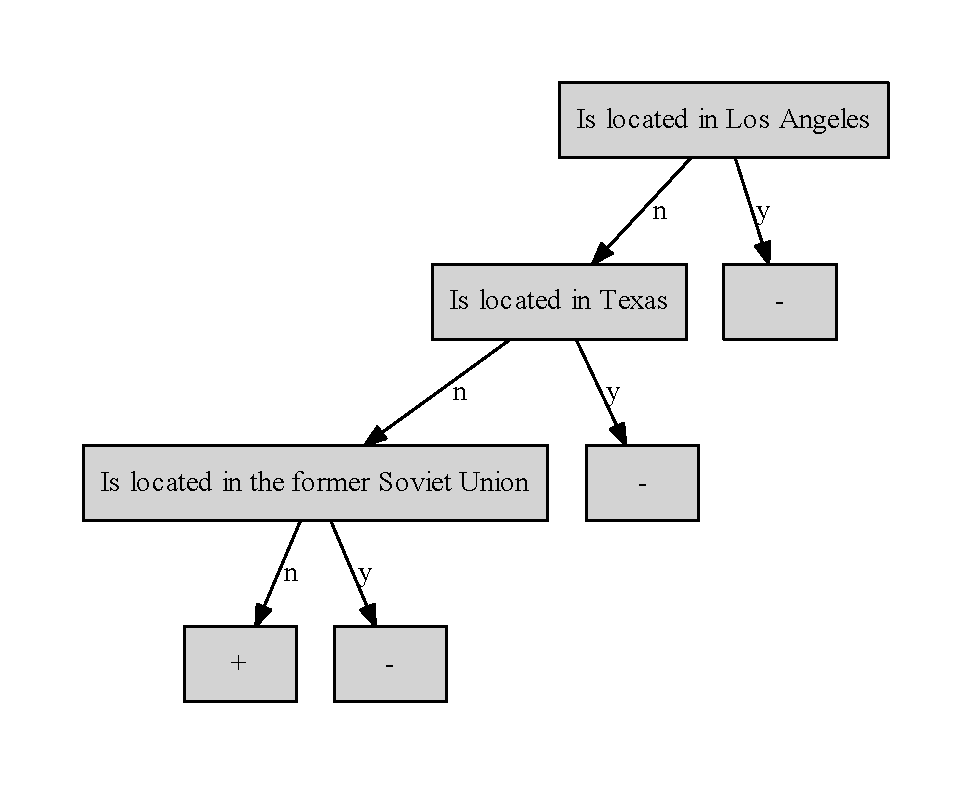
\includegraphics[width=0.8 \linewidth]{level1_good.pdf}
%	\caption{A single level feature regarding nations and organizations with official websites}
%	\label{fig:level1_good}
%\end{figure}

%\begin{figure}[]
%	\centering
%	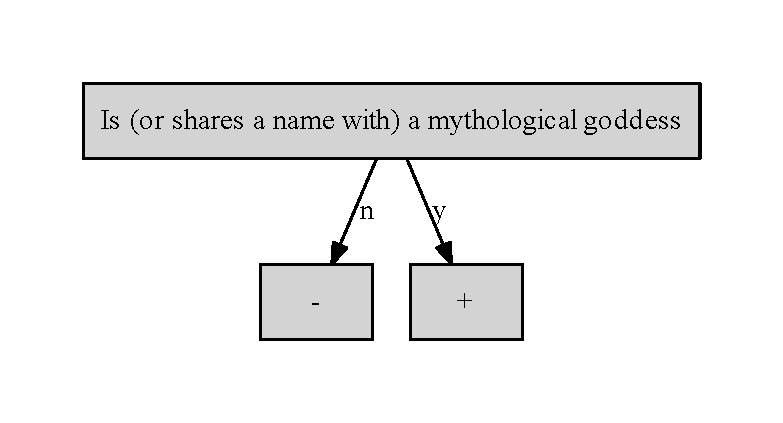
\includegraphics[width=0.6 \linewidth]{level1_simple.pdf}
%	\caption{A single level feature regarding people (real or fictional)}
%	\label{fig:level1_simple}
%\end{figure}

%\begin{figure}[]
%	\centering
%	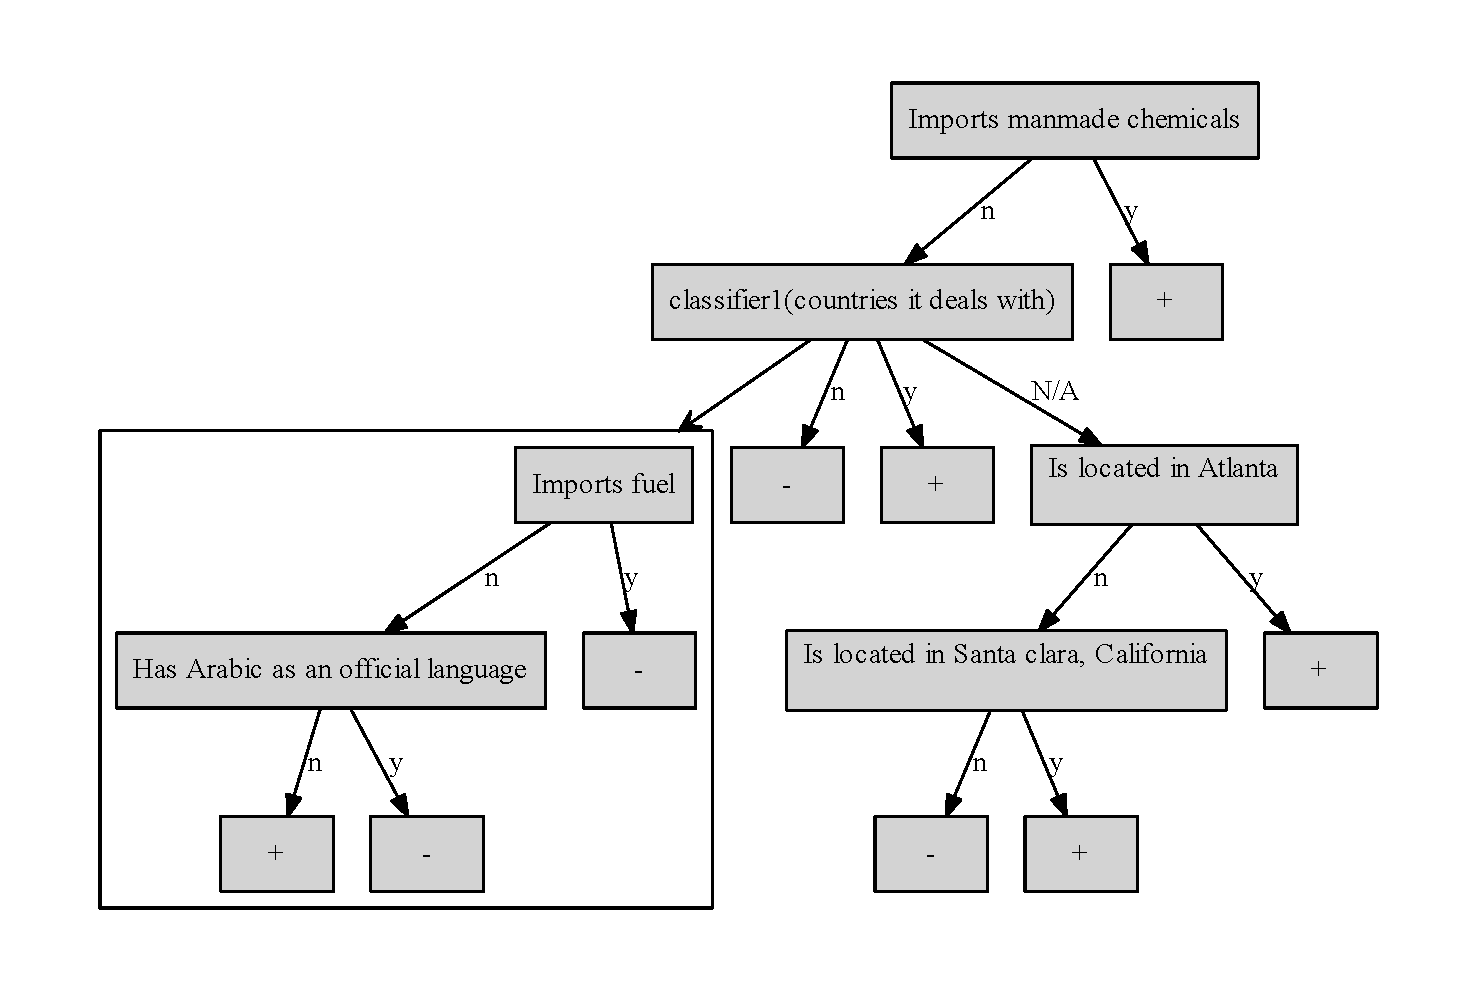
\includegraphics[width=\linewidth]{level2_tree.pdf}
%	\caption{A two level feature regarding countries and organizations}
%	\label{fig:level2_tree}
%\end{figure}

%\begin{figure}[]
%	\centering
%	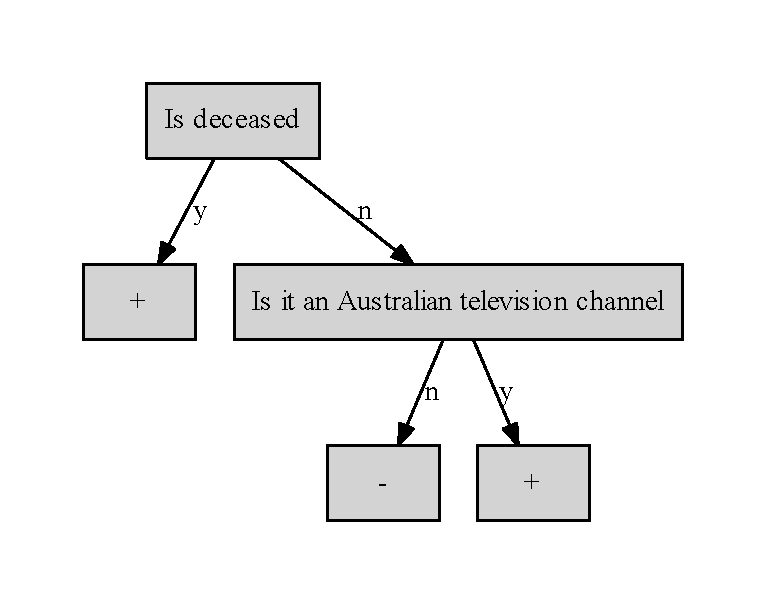
\includegraphics[width=0.6 \linewidth]{weird_trees.pdf}
%	\caption{A single level feature regarding things with a grammatical gender}
%	\label{fig:weird_trees}
%\end{figure}


\section{Related Work}
One of the earliest methods of utilizing relational information is \emph{Inductive Logic Programming(ILP)} \cite{quinlan1990learning,muggleton1991inductive}, which induces a set of first-order formulae that define a good separation of the given training set.
Following this work, Relational Learning - techniques designed to utilize relational databases, have become increasingly prevalent. One such technique is that of View Learning \cite{davis2005view}, which generated new tables from existing ones, effectively performing feature generation for relational methods.
Unlike View Learning and other Relational Learning methods, our approach constructs a new learning problem in a new domain using the existing problem as a guide. Due to this distinction, we essentially try to re-think about our problem from a new direction, rather than trying to fit increasingly less connected entities to the original problem. Furthermore, the ability of our approach to locate locally beneficial features which may be difficult to otherwise detect is invaluable. Finally, we note that the use of decision trees during the feature generation process allows for a natural method by which to filter out features even before applying feature selection mechanisms.

One major attempt at adding relational knowledge to traditional induction algorithms was \emph{propositionalization} \cite{kramer2000bottom}, which allows an unsupervised creations of first-order predicates which can then be used as features for propositional methods. A major setback of this process is that it generates an impractically large number of features, most of which irrelevant.  To this end, \emph{upgrade} methods such as ICL \cite{van2001upgrade} and SGLR \cite{popescul200716} were suggested, where instead of creating predicates a-priori, feature generation is performed during the training phase, in a more structured manner. While upgrade approaches bear some similarities to our approach, there are several critical differences, the key of which is the ability to more easily locate complex features through the use of existing induction algorithms.

Recently, there has been a strong trend of utilizing \emph{Deep Learning} \cite{lecun1998gradient,bengio2009learning} as a feature generation technique. Good examples of this can be seen in FEX \cite{plotz2011featurefull} and DBN2 \cite{kim2013deepfull}. These methods essentially form combinations and transformations on pre-defined features in a semi-supervised manner, thus yielding new, more predictive features. Our approach can be seen as a variation on the same concept, with the transformations being the construction of recursive learning problems, and the combinations being the classifiers constructed in the new problem domain. Our approach differs from those rooted in Deep Learning in both the use of relational data to enrich the feature space, and in that we allow more complex combinations in general.

\section{Conclusions}
%finishing up and summary
We presented a novel new approach to feature generation using relational data, based on constructing and solving new learning problems in the relational domain. While we focused on applying this approach to text categorization problems, it is important to note that it is applicable to any classification problem where feature values are categorical and have semantic meanings, such as drug names, cities and so on. While there is no simple way to generalize this approach to numeric features, we believe there are numerous domains where feature values do have semantic meaning, even excluding text categorization problems.

While our approach only generates binary features, aggregation based techniques such as those used in SGLR apply here as well. A major source for potential improvement is the subject of matching values to semantic objects. Given the major advances in the field of Wikification \cite{bunescu2006using} in general and Entity Linking\cite{rao2013entity} in particular, these approaches can be used to link the initial text to entities within the semantic data without losing information, which may lead to better results.

Another major potential avenue for improvement is to use the techniques discussed in the algorithmic section as a way to directly label entities within the semantic net, which yields a Collective Classification \cite{kajdanowicz2013collective} problem in the semantic domain. Solving this learning problem in turn gives us a feature which can then be applied to the non-relational problem domain.

%\appendix
\begin{appendices}
	\section{FEAGURE pseudocode} \label{app:2}
	
	\begin{algorithm}[H]
		\caption{FEAGURE}
		\label{code2}
		\small
		$S=\{(o_{i},y_{i})\}$- set of labeled objects. We will mark $Obs$ the objects and $y$ the appropriate labels.
		
		$F$- A set of feature-functions.
		
		$R$- A set of relations.
		
		$d$- Maximum depth.
		
		min-leaf- Minimum Leaf Size. For clarity we assume this is constant for all recursive levels.
		
		\begin{algorithmic}
			\Function{FEAGURE}{S, F, R, d, min-leaf} %pick feature, split until min-leaf
				\If {$|S|\leq min-leaf$}
					\State
					\Return Leaf \Comment{We pick features until the tree is too small}
				\EndIf
				\State nf, feature= \Call{RI-ChooseFeature}{S, F, R, d, min-leaf}
				\State \Call{output}{nf}
				\State
				\Return \Call{splitTreeByFeature}{feature, S}
			\EndFunction
			\Function{RI-ChooseFeature}{S, F, R, d, min-leaf}
			\If {$d = 0$}
				\State
				\Return \Call{constructClassifier}{S,F} \Comment{Can use any traiditional learning algorithm}
			\EndIf
			\State addedFeatures= $\{\}$
			\While {resources not exhausted, new relevant features exist}
				\State feature= \Call {pickFeature}{S,F} \Comment{Weighted sampling based on information gain}
				\State newObs= feature(Obs)
				\State newY= \Call {label}{S,newObs} \Comment{In our example, by majority vote}
				\State newF= $\{R_{i}(newObs)|R_{i}\in R, newObs\cap Dom_{i}\neq\emptyset\}$ \Comment{A feature function per relevant relation}
				\State S'= (newObs,newY)
				\State newClassifer= \Call {FEAGURE}{S', newF, R, $d-1$, min-leaf}
				\State f= function(x): return newClassifer(feature(x))
				\If {\Call{InfoGainratio}{f, S} $\geq$ \Call{BestInfoGainratio}{F, S}}
					\State addedFeatures= addedFeatures$\cup \{f\}$ \Comment{A feature passed our threshold, so we add it}
				\EndIf
			\EndWhile
			\State
			\Return addedFeatures, \Call{findBestFeatureByInfoGain}{F$\cup$addedF, S}
			\EndFunction
			
		\end{algorithmic}
	\end{algorithm}
	
\end{appendices}

%\clearpage
\vskip 0.2in
\bibliographystyle{theapa}
\bibliography{document}
%\bibliographystyle{plainnat}
%\bibliography{document}

\end{document} 